\documentclass[12pt]{article}
\usepackage[left=1in,right=1in,top=0.75in,bottom=1in]{geometry} % never use the anysize package!
\usepackage{amsmath, amssymb, fp}
\usepackage{mathpazo}
\usepackage[table]{xcolor}
\usepackage{colortbl}
\usepackage{tabularx}
\usepackage{multirow,multicol}
\usepackage{adjustbox}
\usepackage{morefloats}
\usepackage{tikz}
% \usepackage[firstpage]{draftwatermark}
\usepackage[american, EFvoltages, cuteinductors]{circuitikz}
\usepackage{hyperref}
\usepackage{verbatim}
\usepackage{marvosym}
\usepackage[font=small,labelfont=bf, width=0.9\textwidth]{caption}

\renewcommand*{\thefootnote}{\arabic{footnote}}

\newcolumntype{R}[2]{%
    >{\adjustbox{angle=#1,lap=\width-(#2)}\bgroup}%
    l%
    <{\egroup}%
}

\graphicspath{{./images/}{./soldering/}}

% \SetWatermarkFontSize{5cm}
% \SetWatermarkScale{1}

\fboxsep = 6.0pt
\parskip = 6.0pt
\parindent = 0.0pt
\hfuzz = 18.0pt

% Numerous macros in here:
% tikz stuff and other macros
% Jesse Hamner
% 2013--2024

\usepackage{tabularx}

\newcolumntype{R}[2]{%
    >{\adjustbox{angle=#1,lap=\width-(#2)}\bgroup}%
    l%
    <{\egroup}%
}


% make a few color defs:
\definecolor{rltbrightred}{rgb}{1,0,0}
\definecolor{rltred}{rgb}{0.75,0,0}
\definecolor{rltdarkred}{rgb}{0.5,0,0}
\definecolor{rltbrightgreen}{rgb}{0,0.75,0}
\definecolor{rltgreen}{rgb}{0,0.5,0}
\definecolor{rltdarkgreen}{rgb}{0,0.25,0}
\definecolor{rltbrightblue}{rgb}{0,0,1}
\definecolor{rltblue}{rgb}{0,0,0.75}
\definecolor{rltdarkblue}{rgb}{0,0,0.5}
%\definecolor{webred}{rgb}{0.5,.25,0}
\definecolor{webblue}{rgb}{0,0,0.75}
\definecolor{webgreen}{rgb}{0,0.5,0}
\definecolor{lightgray}{gray}{0.9}
\definecolor{medgray}{gray}{0.6}
\definecolor{footlineblue}{rgb}{0.392,0.706,0.941}
\definecolor{darkgreen}{rgb}{0.00,0.50,0.00}
\definecolor{gray50}{gray}{0.50}
\definecolor{gray95}{gray}{0.95}
\definecolor{webred}{rgb}{0.75,0,0.0}

\renewcommand{\thefootnote}{\fnsymbol{footnote}}
\newcommand{\sep}{1mm}
\newcommand{\negsep}{-4mm}
\newcommand{\widesep}{7mm}
\newcommand{\thisscale}{0.6}
\newcommand{\grr}{\rowcolor{gray!15}}

\newcommand{\+}{\item}		% easier than typing \item a lot
\newcommand{\bi}{\begin{itemize}}
\newcommand{\ei}{\end{itemize}}
\newcommand{\bd}{\begin{description}}
\newcommand{\ed}{\end{description}}
\newcommand{\be}{\begin{enumerate}}
\newcommand{\ee}{\end{enumerate}}
\newcommand{\rr}{\raggedright}

\newcommand{\cb}{\cellcolor{black!35}}

\newcommand{\ckb}{\item[$\square$]} % list checkboxes (requires marvosym)

% A command that makes a uniform box around a paragraph. 
% It's a minipage environment, which means it doesn't support some commands.
\newcommand{\stbox}[2]{
	\begin{center}
	\fbox{
		\begin{minipage}[c]{#1}{
		\noindent #2
		}
		\end{minipage}
	}
	\end{center}
}


% A series of macros that enable programmatic of drawing stylized
% ions, protons, or electrons.
% Supports,  e.g., richer drawings of capacitors or
% current flowing in wires:

\newcommand{\ionradius}{0.06} % TODO should make it possible to change this too

\newcommand{\drawion}[4]{
		\draw [black, very thin] (#1,#2) circle [radius=#3];
		\node[scale=0.3, thick ] at (#1,#2) {#4};
}

\newcommand{\posion}[3]{
		\drawion{#1}{#2}{#3}{$+$}
		}

\newcommand{\negion}[3]{
		\drawion{#1}{#2}{#3}{$-$}
		}

\newcommand{\horizionarray}[4]{
	\newdimen\len
	\len=#1 cm
	\advance\len by -0.4cm
	\drawion{\len}{#2}{\ionradius}{#4}
	\advance\len by 0.15cm
	\drawion{\len}{#2}{\ionradius}{#4}
	\advance\len by 0.15cm
	\drawion{\len}{#2}{\ionradius}{#4}
	\advance\len by 0.2cm
	\drawion{\len}{#2}{\ionradius}{#4}
	\advance\len by 0.15cm
	\drawion{\len}{#2}{\ionradius}{#4}
	\advance\len by 0.15cm
	\drawion{\len}{#2}{\ionradius}{#4}
}

\newcommand{\vertionarray}[4]{
	\newdimen\len
	\len=#2 cm
	\advance\len by -0.4cm
	\drawion{#1}{\len}{\ionradius}{#4}
	\advance\len by 0.15cm
	\drawion{#1}{\len}{\ionradius}{#4}
	\advance\len by 0.15cm
	\drawion{#1}{\len}{\ionradius}{#4}
	\advance\len by 0.2cm
	\drawion{#1}{\len}{\ionradius}{#4}
	\advance\len by 0.15cm
	\drawion{#1}{\len}{\ionradius}{#4}
	\advance\len by 0.15cm
	\drawion{#1}{\len}{\ionradius}{#4}
}



% Nokia 84 x 48 pixel LCD screen (usually model number 5110 or 3310)
\newcommand{\drawnokiagrid}{
\draw[step=1cm,blue!30,very thin] (0,0) grid (6,8);
\foreach \x in {0,1,2,3,4,5}
	\draw (\x cm, 0pt) -- (\x cm, -3pt) node[anchor=north] {$\x$};
\foreach \y in {1,2,3,4,5,6,7,8}
	\draw (0pt, \y cm) -- (-3pt, \y cm) node[anchor=east] {$\y$};
}


% part of the Nokia grid set of commands
\newcommand{\msqo}[3]{
\def\mycmd{#3}

\if\mycmd1
	\msq{#1}{#2}{black!65}
\else
	\msq{#1}{#2}{white}
\fi
}


% part of the Nokia grid set of commands
\newcommand{\msq}[3]{
\edef\myx{#1}
\pgfmathparse{\myx+1.0}
\edef\myxtwo{\pgfmathresult}
\edef\myy{#2}
\pgfmathparse{\myy+1.0}
\edef\myytwo{\pgfmathresult}
\fill[#3] (\myx,#2) rectangle (\myxtwo,\myytwo);}


% part of the Nokia grid set of commands
\newcommand{\mcol}[9]{
\msqo{#1}{#2}{#3}
\msqo{#1}{#4}{#5}
\msqo{#1}{#6}{#7}
\msqo{#1}{#8}{#9}
}


% part of the Nokia grid set of commands
\newcommand{\hexlabel}[5]{
\node[rotate=90] at (0.5,-1) {\Large\texttt{#1}};
\node[rotate=90] at (1.5,-1) {\Large\texttt{#2}};
\node[rotate=90] at (2.5,-1) {\Large\texttt{#3}};
\node[rotate=90] at (3.5,-1) {\Large\texttt{#4}};
\node[rotate=90] at (4.5,-1) {\Large\texttt{#5}};
}



% drawing cubes using TikZ:
\newcommand{\makecube}[2]{
\begin{tikzpicture}[xscale=#2,yscale=#2]
\foreach \x in{0,...,#1}
{   \draw (0,\x ,#1) -- (#1,\x ,#1);
    \draw (\x ,0,#1) -- (\x ,#1,#1);
    \draw (#1,\x ,#1) -- (#1,\x ,0);
    \draw (\x ,#1,#1) -- (\x ,#1,0);
    \draw (#1,0,\x ) -- (#1,#1,\x );
    \draw (0,#1,\x ) -- (#1,#1,\x );
}
\end{tikzpicture}
}


% Draw faux-3D squares or cubes:
\newcommand{\makeplate}[3]{
\begin{tikzpicture}[xscale=#3,yscale=#3]

\foreach \x in {0,...,#1}
{
	\filldraw[gray95, fill=gray95, line width=0.0cm] (0,#1,0) -- (0,#1,#2) -- (#1,#1,#2) -- (#1,#1, 0) -- (0,#1,0) -- cycle;
	\filldraw[gray50, fill=gray50, line width=0.0cm] (#1,#1,0) -- (#1,#1,#2) -- (#1,0,#2) -- (#1,0, 0) -- (#1,#1,0) -- cycle;
}

\foreach \x in{0,...,#1}
{   \draw (0,\x ,#2) -- (#1,\x ,#2);
    \draw (\x ,0,#2) -- (\x ,#1,#2);
	\draw (#1,\x ,#2 ) -- (#1,\x ,0);
    \draw (\x ,#1,#2 ) -- (\x ,#1,0);
}

\foreach \x in {0,...,#2}
{
    \draw(#1,0,\x  ) -- (#1,#1,\x );
    \draw(0,#1,\x  ) -- (#1,#1,\x );
}

\foreach \x in{1,...,#1}
{
\node[align=left] at (\x-0.5,#1-0.5,#2) {\x};
}

\foreach \x in{#1,...,2}
{
\node[align=left] at (0.5,#1-\x+0.5,#2) {\x};
}

%\draw[webred, thick](0,0,0) -- (0,0,#2);
%\draw[webblue, thick](0,0,0) -- (#1,0,0);
%\draw[darkgreen, thick](0,0,0) -- (0,#1,0);

\end{tikzpicture}
}


% Draw a line of faux-3D shaded blocks using TikZ:
\newcommand{\blockline}[2]{
\begin{tikzpicture}[xscale=#2,yscale=#2]

\filldraw[fill=gray95, ultra thin] (0,1,0) -- (0,1,1) -- (#1,1,1) -- (#1,1, 0) -- (0,1,0) -- cycle;
\filldraw[fill=gray50, ultra thin] (#1,1,0) -- (#1,1,1) -- (#1,0,1) -- (#1,0, 0) -- (#1,1,0) -- cycle;

\draw (0,1,0 ) -- (#1,1,0); % top line
\draw (#1,1,1) -- (#1,1,0);
\draw (#1,0,1) -- (#1,1,1);
\draw (0,1, 1) -- (#1,1,1);
\draw (0,0,1 ) -- (#1,0,1);

\foreach \x in{0,...,#1}
{   
    \draw (\x ,0,1) -- (\x ,1,1 ); % straight vertical lines    
    \draw (\x ,1,1) -- (\x ,1,0 );
}

\foreach \x in{1,...,#1}
{
	\node[align=left] at (\x-0.5,0.5,1) {\x};
}

\end{tikzpicture}
}


% make a blank line under which, e.g., someone could write an unknown answer:
\newcommand{\makeblank}[1]{
\underline{\makebox[#1][l]{}}
}


% tilt the text atop a table row at an angle:
\newcommand*\rot{\multicolumn{1}{R{55}{1.2ex}}}% no optional argument here, please!


\newcommand{\adderblock}[3]{

	\begin{scope}

	\draw (0,#1)
	  [xshift = 2.5cm]
	  node[one bit adder, scale=0.75](fa#2){}
	  node[xshift=0.75cm, yshift=1cm](fa#2carrylabel){\footnotesize $Carry_#3$}
  	  node[ocirc, xshift=1.5cm, label={[label distance=0mm]0:$Sum_#3$}](fa#2sum){}
	;

    \draw (0.5,#1)
 	  [yshift=-0.65cm] 
	  node[american xor port](axorb#2){}
	  node[ocirc, xshift = -2.2cm, yshift = -0.28cm](axorb#2node){}
   	  node[xshift = -2.6cm, yshift = 0mm](){{\color{red}$A_{#3}$}}
	  node[xshift = 0.2cm, yshift = 6mm] {{\footnotesize{$XOR_{#3}$}}}
   	  node[ocirc, xshift = -4.5cm, yshift = 0.32cm](m#2node){}
	  node[xshift = -4.0cm, yshift = 0.6cm, color=rltred]{\color{rltred}$M_{#3}$}
	;
 
    \draw (0,#1)
	  [yshift=0.65cm]
	  node[ocirc, xshift = -2.0cm](b#2node){}
   	  node[xshift = -2.3cm, yshift = 3mm](){{\color{blue}$B_{#3}$}}
    ;
  
    \draw (0,#1)
	  [color=blue] 
	  (b#2node) -- (fa#2.lpin 1) 
	;
  
    \draw
	  [color=rltred] 
	  (m#2node) -- (axorb#2.in 1) 
	;

    \draw (0,#1)
	  (axorb#2node) -- (axorb#2.in 2)
	  (fa#2.rpin 1) -- (fa#2sum)
	;
	
    \draw(0, #1)[color=brown, very thick]
      (axorb#2.out) -- (fa#2.lpin 2)
    ;
    
  \end{scope}
}



% Half Adder Symbol:
\newcommand{\halfadder}{
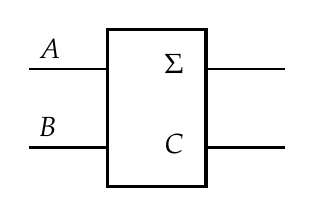
\begin{tikzpicture}

\draw [very thick] (0,0) -- (1.25,0) -- (1.25,2) -- (0,2) -- cycle;
\draw [thick] (-1,0.5) -- (0,0.5);
\draw [thick] (-1,1.5) -- (0,1.5);
\draw [thick] (1.25,0.5) -- (2.25,0.5);
\draw [thick] (1.25,1.5) -- (2.25,1.5);

\node[xshift=-10mm, yshift=20mm, anchor= north west] {$A$};
\node[xshift=-10mm, yshift=10mm, anchor= north west] {$B$};
\node[xshift=6mm, yshift=18mm, anchor= north west] {$\Sigma$};
\node[xshift=6mm, yshift=8mm, anchor= north west] {$C$};

\end{tikzpicture}
}


% Full Adder Symbol:
\newcommand{\fulladder}{
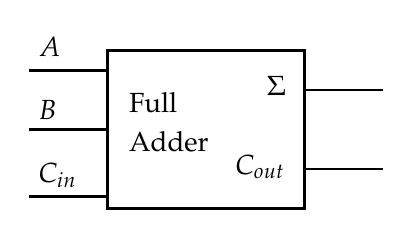
\begin{tikzpicture}

\draw [very thick] (0,0) -- (2.5,0) -- (2.5,2) -- (0,2) -- cycle;
\draw [thick] (-1,0.15) -- (0,0.15);
\draw [thick] (-1,1.0) -- (0,1.0);
\draw [thick] (-1,1.75) -- (0,1.75);

\draw [thick] (2.5,0.5) -- (3.5,0.5);
\draw [thick] (2.5,1.5) -- (3.5,1.5);

\node[xshift=-10mm, yshift=23mm, anchor= north west] {$A$};
\node[xshift=-10mm, yshift=15mm, anchor= north west] {$B$};
\node[xshift=-10mm, yshift=7mm, anchor= north west] {$C_{in}$};

\node[xshift=19mm, yshift=18mm, anchor= north west] {$\Sigma$};
\node[xshift=15mm, yshift=8mm, anchor= north west] {$C_{out}$};
\node[xshift=1.5mm, yshift=16mm, anchor= north west] {Full};
\node[xshift=1.5mm, yshift=11mm, anchor= north west] {Adder};

\end{tikzpicture}
}



% reset with initially Q = 0, ~Q = 1
\newcommand{\actionreset}{
  \renewcommand{\clockcolor}{hot}
  \renewcommand{\jinput}{ground}
  \renewcommand{\kinput}{hot}
  \renewcommand{\joutput}{hot}
  \renewcommand{\koutput}{hot}
  \renewcommand{\qoutput}{ground}
  \renewcommand{\notqoutput}{hot}
  \renewcommand{\nandonecolor}{on}
  \renewcommand{\nandtwocolor}{on}
  \renewcommand{\nandthreecolor}{off}
  \renewcommand{\nandfourcolor}{on}
  \renewcommand{\jinputpulse}{thin}
  \renewcommand{\kinputpulse}{very thick}
}


% set with initially Q = 0, ~Q = 1
\newcommand{\actionset}{
  \renewcommand{\clockcolor}{hot}
  \renewcommand{\jinput}{hot}
  \renewcommand{\kinput}{ground}
  \renewcommand{\joutput}{hot}
  \renewcommand{\koutput}{hot}
  \renewcommand{\qoutput}{hot}
  \renewcommand{\notqoutput}{ground}
  \renewcommand{\nandonecolor}{on}
  \renewcommand{\nandtwocolor}{on}
  \renewcommand{\nandthreecolor}{on}
  \renewcommand{\nandfourcolor}{off}
  \renewcommand{\jinputpulse}{very thick}
  \renewcommand{\kinputpulse}{thin}

}


% no clock signal with initially Q = 1, ~Q = 0 and no inputs
\newcommand{\noclocknoinputs}{
  \renewcommand{\clockcolor}{ground}
  \renewcommand{\jinput}{ground}
  \renewcommand{\kinput}{ground}
  \renewcommand{\joutput}{ground}
  \renewcommand{\koutput}{hot}
  \renewcommand{\qoutput}{hot}
  \renewcommand{\notqoutput}{ground}
  \renewcommand{\nandonecolor}{on}
  \renewcommand{\nandtwocolor}{on}
  \renewcommand{\nandthreecolor}{on}
  \renewcommand{\nandfourcolor}{off}
  \renewcommand{\jinputpulse}{thin}
  \renewcommand{\kinputpulse}{thin}

}

% no clock signal with initially Q = 0, ~Q = 1 and SET input only
\newcommand{\noclockset}{
  \renewcommand{\clockcolor}{ground}
  \renewcommand{\jinput}{hot}
  \renewcommand{\kinput}{ground}
  \renewcommand{\joutput}{hot}
  \renewcommand{\koutput}{hot}
  \renewcommand{\qoutput}{hot}
  \renewcommand{\notqoutput}{ground}
  \renewcommand{\nandonecolor}{on}
  \renewcommand{\nandtwocolor}{on}
  \renewcommand{\nandthreecolor}{on}
  \renewcommand{\nandfourcolor}{off}
  \renewcommand{\jinputpulse}{very thick}
  \renewcommand{\kinputpulse}{thin}

}


% no clock signal with initially Q = 0, ~Q = 1 and RESET input only
\newcommand{\noclockreset}{
  \renewcommand{\clockcolor}{ground}
  \renewcommand{\jinput}{ground}
  \renewcommand{\kinput}{hot}
  \renewcommand{\joutput}{hot}
  \renewcommand{\koutput}{hot}
  \renewcommand{\qoutput}{hot}
  \renewcommand{\notqoutput}{ground}
  \renewcommand{\nandonecolor}{on}
  \renewcommand{\nandtwocolor}{on}
  \renewcommand{\nandthreecolor}{on}
  \renewcommand{\nandfourcolor}{off}
  \renewcommand{\jinputpulse}{thin}
  \renewcommand{\kinputpulse}{very thick}
}

%%%%%%%%%%%%%%%%%%%%%%%%%%%%%%%%%%%%%%%%%%%%%%%%%%%%%%%%%%%%%%%%
\begin{document}
%%%%%%%%%%%%%%%%%%%%%%%%%%%%%%%%%%%%%%%%%%%%%%%%%%%%%%%%%%%%%%%%

\thispagestyle{empty}

\title{Introducing Computer Theory to Fourth Graders}
\author{Jesse Hamner}
\date{2017--2022\\
% \vspace{0.15in}
% \begin{quote}
% \centering
% {\color{red}\emph{Draft Copy: Do not cite.}} % use version number later
% \end{quote}
}

\maketitle

\begin{abstract}
Kids are using technology that is intuitive to control, but entirely opaque to the children's understanding. Why do computers work? How do computers count and add numbers? What makes transistors so important? How can we put transistors together to make a computer? 

This workshop aims to produce a short course of study for third to sixth graders, that takes about three afternoons to complete. Children are introduced to math concepts fundamental to the study of computing such as binary counting, exponentiation, basic electronics theory, and computing logic. Several hands-on projects are included in the text and can enhance the students' learning while breaking up the ``lecture'' format of the workshop.

\bigskip

\noindent\textbf{Keywords:} STEM; education; computing theory; logic; electronics theory; elementary education; logic gates; science experiments.

\bigskip

\noindent All source code for this document are available at {\color{webblue}\href{https://github.com/jessehamner/TechMillForKids}{the project's GitHub page}}.

\end{abstract}

\vfill

\begin{center}
\includegraphics[scale=1.0]{by-nc-nd.png}

This work is licensed under a {\color{webblue}\href{https://creativecommons.org/licenses/by-nc-sa/4.0/}{Creative Commons Attribution-NonCommercial-ShareAlike 4.0 International License.}}

% Attribution-NonCommercial-ShareAlike 4.0 International (CC BY-NC-SA 4.0)
\end{center}

% Table of Contents:
%---------------------------
\newpage
\tableofcontents

\vfill

\clearpage
%---------------------------


% Introduction:
%---------------------------
\newpage
\section{Introduction}

This workshop is going to help you learn about computers -- but not how to \emph{use} computers. Rather, when we are finished, you will understand a little bit about how and why computers really do work and get answers to math problems. To get to that goal, you'll need to learn some new topics in math, and learn about electricity. You'll also need to learn about basic \emph{electronic components}, too. These are the small pieces that are used together in \emph{circuits} to do useful things with electricity. When assembled, circuits (whether simple or complex) enable electricity to do all the things we can make electricity do, like light our homes, play music on the radio, find directions with a GPS, run a gasoline engine, or show you a web page.

Computers are wonderful, multipurpose machines that take in data, store data, and change data according to instructions that are provided to the computer. But computers can't add or subtract the way you do. They can't read the way you do. They don't think. Really,  \emph{they only do math.} Everything computers do is controlled by a series of instructions that \emph{all boil down to math and logic,} even if it looks like magic. The way computers do all the things they do can always be described as a series of instructions. Each of these actions can be performed by some combination of special circuit types, and each circuit is made up of basic electronic components. You can learn enough about each basic component to understand what it does, without needing to do a bunch of math. And, you can understand all the individual instructions, even if you don't want to build your own computer!

Ultimately this workshop will make it possible for you to make, from the most basic electronic components, a simple digital computer that can add two numbers and correctly display the result, or tell you whether or not two numbers are equal. Along the way you'll see how each piece works, and how to put the pieces together. Some workshops will also teach you how to solder components, so you can actually \emph{make} some of the building blocks of computers. There are follow-on discussions about other topics like subtraction and using circuits to store information so a computer can use it later.

This time together should be fun! You can help make it fun for everyone by asking questions and by telling the instructor what you think about the parts of this course. It's not easy to teach this material, so your feedback will help the authors improve this course over time, as the feedback from many people has already improved this workshop.

I'm so glad you're interested in computers. It makes me feel good when people learn things and have fun with this course. Thank you!
\bigskip

\noindent Jesse Hamner, PhD\\
\noindent 2018--2020\\

%---------------------------


% Bases, exponents, decimal and binary math
%---------------------------
\newpage
\section{Decimal and Binary Math}

The next few sections introduce some math ideas that may or may not be familiar to you. In order to really understand how computers work, you need to understand several math concepts that are not hard, but may be unfamiliar. The first concept is the \emph{exponent}. 

\subsection*{Bases and Exponents}

Exponentiation is a mathematical operation, written as $b^n$, involving two numbers, the base, $b$, and the exponent, $n$. Exponentiation means ``repeated multiplication of the base." 

\noindent That is, $b^n$ is the product of multiplying the base number $n$ times:


\begin{equation*}
b^{n}=\underbrace {b\times \cdots \times b} _{n}
\end{equation*}

\noindent In this case, $b^n$ is called the ``\emph{n-th} power of b", or ``b raised to the power n." So 3 to the 4\textsuperscript{th} power looks like this: 

\begin{equation*}
3^4 ~=~ 3 \times 3 \times 3 \times 3 ~=~ 9 \times 9 ~=~  81
\end{equation*}



Put another way: the exponent is a number, smaller and on the upper right hand side of a number, that means ``multiplying a number times itself zero times, once, or more than once" depending on whether the number is 0, 1, 2, or another number (written $n$ in the description above). It is possible to use fractions as exponents, but we won't talk about that here.

The base can be any number, though most people think most easily in base-10. So in base-10, 10 to the power 2, or 10 to the second power, means $10 \times 10$. 

\subsection*{Order of Magnitude (Columns)}

When counting up from zero, by one, in base 10, you eventually get to 9. In order to count any higher, you must ``carry the one" over to the next column and reset the counter in the ``ones" column (the place that counts by one, from zero to nine). When you move from the ``\emph{ones}'' column to the ``\emph{tens}'' column, the next column to the left represents the next \emph{order of magnitude} of the base. ``Magnitude" means ``size", and in math, it means, specifically, moving from counting by one number (the base) to counting by the base times itself -- first twice, then three times, then more. For base-10, you count from 0 to 9 in the right-most column, then from 10 to 90 in the next column to the left, then from 100 to 900 in the next column to the left, then from 1000 to 9000, and so on. Each time the counter gets full (reaches 9), you cannot represent any more of the quantity being counted without moving to the next largest order of magnitude. That is, if your display only shows two digits, once you count past 99, you have no idea is the number is 0, or 100, or 200, or 900, or ten thousand, or 4 billion.



\newpage
\subsection*{Squares}

Shapes that are squares have four sides with the same length; that is, the length and width are the same. \emph{Squaring a number} is multiplying the number times itself, just like, in a square, both sides have the same length. The most common way you will see a ``squared number" described is with a little 2 up above the number, like  $2^2$, or $3^2$, or $10^2$. That smaller `2' is the exponent, that we discussed above.

\medskip

Squaring the number 10 (that is, multiplying ten times itself) gets: $10 \times 10 = 100$

\bigskip

\begin{tabular}{l m{0.75in} l l }

\blockline{1}{0.5} & $1 \times 1 = $ & \blockline{1}{0.5} & $=1^2$ \\
\\
\blockline{2}{0.5} & $2 \times 2 = $ & \makeplate{2}{1}{0.5} & $=2^2$ \\
\\
\blockline{3}{0.5} & $3 \times 3 = $ & \makeplate{3}{1}{0.5} & $=3^2$\\
\\
\blockline{4}{0.5} & $4 \times 4 = $ & \makeplate{4}{1}{0.5} & $=4^2$ \\
\\
\blockline{5}{0.5} & $5 \times 5 = $ & \makeplate{5}{1}{0.5} & $=5^2$ \\
\\
\blockline{6}{0.5} & $6 \times 6 = $ & \makeplate{6}{1}{0.5} & $=6^2$ \\

\end{tabular}

\newpage

\subsection*{Cubes}

Cubes have the same length side, on each of six sides, in \emph{three} dimensions. When cubing a number, you are multiplying the number times itself, and then multiplying it times itself \emph{again}, because all three sides are the same (they have the same value). The most common way you will see a ``cubed number" described is with a little 3 up above the number, like  $2^3$, or $3^3$, or $10^3$. As above, the exponent tells you how many times you multiply the number times itself (here, that means three times).

\medskip

Cubing the number 10 gets: $10 \times 10 \times 10 = 1000$

\bigskip

\begin{tabular}{m{1.1in} m{1.0in} m{1.45in} m{1.9in}}

\blockline{1}{0.5} & $1 \times 1 \times 1 = $ & \blockline{1}{0.5} & One times itself is one.\\
\\
\blockline{2}{0.5} & $2 \times 2\times 2 = $ & \makeplate{2}{2}{0.5} & Two sets of four, or \newline$4+4$ (that is, $2^2 + 2^2$) \\
\\
\blockline{3}{0.5} & $3 \times 3 \times 3 = $ & \makeplate{3}{3}{0.5} & Three sets of nine, or \newline$9+9+9$\newline Put another way:\newline $9 \times 3 = 27$ \\
\\

\blockline{4}{0.5} & $4 \times 4 \times 4 = $ & \makeplate{4}{4}{0.5} & Cubes get big quickly---\newline Here's four sets of 16. \newline$16 \times 4 = 64$ \\
\\

\blockline{5}{0.5} & $5 \times 5 \times 5 = $ & \makeplate{5}{5}{0.5} & Five sets of 25. \newline$25 \times 5 = 125$ \\
\\


\end{tabular}

\newpage

\subsection*{Multipliers and Prefixes}

In systems of measurement, when talking about, say, weight, height, or pressure, there are base units and there are ways to refer to these base units in large multiples, or in tiny fractions. You're probably a little taller than one \emph{meter} in height. And it takes one hundred \emph{centimeters} to add up to one meter. The prefix ``centi-" means it takes one hundred of \emph{these} to add up to one of the \emph{base unit}, which in this case is a meter.

The same goes for weight. You probably weigh between 20 and 40 \emph{kilograms}. The prefix ``{kilo-}'' means \emph{one thousand} of whatever the base unit is. Put another way, grams are pretty small amounts of weight, so measuring things like people or cars is impractical if we use grams, because cars weigh millions of grams. Medicines, on the other hand,  are usually measured in quantities called \emph{milligrams} -- each milligram is only $\frac{1}{1000}$ (one one-thousandth) of a gram. Don't be confused into thinking ``milli-" means ``million'' --- ``mega" means ``million.''

When thinking about computers, we hear terms that are often expressed as multiples of things like memory and storage capacity. A kilobyte is 1,000 bytes (a \emph{byte} is 8 individual bits, and each bit is the smallest unit of computing -- it can only represent 1 or 0). A megabyte is 1,000 kilobytes (or, 1,000,000 bytes). A gigabyte is one \emph{billion} bytes, and a terabyte is one \emph{trillion} bytes. 


\newpage
\subsection*{Representing Numbers in Decimal}

\emph{Decimal} means ``with tens". You've always been taught to count in the decimal system -- by ten. When you are counting by ones, once you get past 9, you reset the right-most number to zero and add that ten to the next column, which is the \emph{tens} column (so you only increment that counter by one, since you are adding \emph{one} ``ten'' to the total). Once you fill up 9 ``tens" (90) and count up past 9 in the ``ones'' column (that is, you add one to 99), you have to set the ones column and the tens column to zero, and add one to the ``hundreds'' column. You \emph{carry} the ten to the left from the ones, and carry the hundred to the left, to the next-largest set of tens. One hundred is ten tens, one thousand is 100 tens, and so forth.

\noindent It looks like this:
\bigskip

\begin{tabular}{l l l l l | l r }
\rot{ten thousands} & \rot{thousands} & \rot{hundreds} & \rot{tens} & \rot{ones} & \multicolumn{2}{c}{Number} \\
\hline
{\color{lightgray}0} & {\color{lightgray}0} & {\color{lightgray}0} & {\color{lightgray}0} & 0 && 0 \\
{\color{lightgray}0} & {\color{lightgray}0} & {\color{lightgray}0} & {\color{lightgray}0} & 1 && 1 \\
{\color{lightgray}0} & {\color{lightgray}0} & {\color{lightgray}0} & {\color{lightgray}0} & 2 && 2 \\
{\color{lightgray}0} & {\color{lightgray}0} & {\color{lightgray}0} & {\color{lightgray}0} & 3 && 3 \\
{\color{lightgray}0} & {\color{lightgray}0} & {\color{lightgray}0} & {\color{lightgray}0} & 4 && 4 \\
{\color{lightgray}0} & {\color{lightgray}0} & {\color{lightgray}0} & {\color{lightgray}0} & 5 && 5 \\
{\color{lightgray}0} & {\color{lightgray}0} & {\color{lightgray}0} & {\color{lightgray}0} & 6 && 6 \\
{\color{lightgray}0} & {\color{lightgray}0} & {\color{lightgray}0} & {\color{lightgray}0} & 7 && 7 \\
{\color{lightgray}0} & {\color{lightgray}0} & {\color{lightgray}0} & {\color{lightgray}0} & 8 && 8 \\
{\color{lightgray}0} & {\color{lightgray}0} & {\color{lightgray}0} & {\color{lightgray}0} & 9 && 9 \\
{\color{lightgray}0} & {\color{lightgray}0} & {\color{lightgray}0} & 1 & 0 && 10 \\
\end{tabular}
\bigskip

When you get to the bottom of the column, you re-set the counter for that column to zero, and add one to the next column over (carry). So you go from 9 to 10, or 19 to 20, or 99 to 100. So any column can only hold between 0 and 9, before you have to carry over to the next \emph{order of magnitude}, which for a decimal system is \emph{ten times the size of one step in the column}. So when you run out of room for the ones column, you go to the \emph{tens} column, which contains ten times as many units as any single step (from 1 to 2, or from 8 to 9) in the column to the right of it. When you run out of room in the column, you have to carry to the next order of magnitude. You go from the ones, to the tens, to the hundreds (100 is $10 \times 10$), to the thousands (1000 is $10 \times 100$), and so on.

To express a number, we count up the amount of each order of magnitude and add them all together. The number 628 is made of $(6 \times 100) +  (2 \times 10) +  (8 \times 1)$, for instance.

\newpage

Here are a few examples of numbers expressed in columns. For each one, you count up how many units in the column exist, then count them for each order of magnitude, and add each value together to get the number being described:

\bigskip
\begin{tabular}{p{2.7in} | l l   l l l l | l l r }
\hline
\textbf{Text Description} & & \rot{ten thousands} & \rot{thousands} & \rot{hundreds} & \rot{tens} & \rot{ones} && \multicolumn{2}{c}{\textbf{Number}} \\[\sep]
\hline
& && & & & & &&\\[-2mm]

no ten-thousands, no thousands, no hundreds, no tens, and no ones   && {\color{lightgray}0} & {\color{lightgray}0} & {\color{lightgray}0} & {\color{lightgray}0} & 0 &&& 0 \\[\widesep]
no ten-thousands, no thousands, no hundreds, no tens, and one ones   && {\color{lightgray}0} & {\color{lightgray}0} & {\color{lightgray}0} & {\color{lightgray}0} & 1 &&& 1 \\[\widesep]
no ten-thousands, no thousands, no hundreds, no tens, and two ones  && {\color{lightgray}0} & {\color{lightgray}0} & {\color{lightgray}0} & {\color{lightgray}0} & 2 &&& 2 \\[\widesep]
no ten-thousands, no thousands, no hundreds, three tens, and no ones && {\color{lightgray}0} & {\color{lightgray}0} & {\color{lightgray}0} & 3 & 0 &&& 30 \\[\widesep]
no ten-thousands, no thousands, four hundreds, no tens, and no ones && {\color{lightgray}0} & {\color{lightgray}0} & 4 & 0 & 0 &&& 400 \\[\widesep]
no ten-thousands, no thousands, five hundreds, five tens, and five ones && {\color{lightgray}0} & {\color{lightgray}0} & 5 & 5 & 5 &&& 555 \\[\widesep]
no ten-thousands, six thousands, five hundreds, no tens, and two ones && {\color{lightgray}0} & 6 & 5 & 0 & 2 & & & 6502 \\[\widesep]
six ten-thousands, eight thousands, no hundreds, three tens, and no ones && 6 & 8 & 0 & 3 & 0 & & & 68030 \\[\widesep]
\hline
\end{tabular}


\bigskip


\stbox{6.0in}{\emph{Exercise:} What if, in the above table, you counted past 99,999? What number would you see? That is, what do you see if there is not a ``hundred-thousands" column? What happened to the hundred thousand that should be counted? Do you need to know how many hundred thousands are in the number? How would you handle the need for a larger number, if you have it? (Introduces the concept of \emph{overflow}.)}


\newpage
\subsection*{Representing Numbers in Binary}

Computers only understand ``1'' and ``0'' -- because it can sense the electricity in a wire that is either \emph{on} (having a detectable voltage greater than zero) or \emph{off} (having a reference voltage that is basically at ``zero volts", or ``ground."). That means that a computer, in order to add, subtract, or store information, has to express \emph{literally anything and everything it can handle} in terms of either ones or zeroes. This system is called \emph{binary}, because computers only understand two ``states" -- on, or off. Instead of ``base-10" counting (where moving to the next column happens when you pass 9), binary is ``base-2'' counting; the numbers move to the next column when the number passes 1---because {\color{webblue}\href{https://www.youtube.com/watch?v=MOn_ySghN2Y}{there's no such number as ``two''}} if you're a computer!

In order to add numbers in binary, we can't count to ten. We must count to one, and then, if the resulting number is greater than one, carry the digit to the next column. Counting in binary is interesting because it is different, and because it introduces us to a new way of doing math.

In order to add two numbers, computers have to do the following:
\be
\+ store each number in a binary format;
\+ compare each column (ones, twos, fours, eights, etc.) of each number and see if the numbers in that column add up to more than one;
\+ carry the ``one'' to the next column (the next \emph{order of magnitude}, which is two times the previous column). That is, if the number goes from one to two, the ``one" will go to zero and the ``two" will be moved -- and added -- to the next column over to the left;
\+ keep on adding and carrying digits until the addition is complete;
\+ count up the values of each order of magnitude (either one, or none) and add them together; and
\+ report the new number as a [binary] result.
\ee


\begin{minipage}[c]{6.5in}
\begin{center}
\textbf{Binary and decimal representation for each number from 0 to 15:}

\smallskip
\begin{tabular}{p{1.25in} | p{0.10in} p{0.10in} p{0.10in} p{0.10in} | l r}
\hline\\[\negsep]
\textbf{Description} & \rot{eights} & \rot{fours} & \rot{twos} & \rot{ones} && \textbf{{\color{webblue}base 10}}\\[\sep]
\hline\\[\negsep]
$0 + 0 + 0 + 0$   & 0 & 0 & 0 & 0 && {\color{webblue}0} \\

\grr
$0 + 0 + 0 + 1$ & 0 & 0 &  0 & 1 && {\color{webblue}1} \\

$0 + 0 + 2 + 0$   & 0 & 0 & 1 & 0 && {\color{webblue}2} \\

\grr
$0 + 0 + 2 + 1$   & 0 & 0 & 1 & 1 && {\color{webblue}3} \\

$0 + 4 + 0 + 0$   & 0 & 1 & 0 & 0 && {\color{webblue}4} \\

\grr
$0 + 4 + 0 + 1$   & 0 & 1 & 0 & 1 && {\color{webblue}5} \\

$0 + 4 + 2 + 0$   & 0 & 1 & 1 & 0 && {\color{webblue}6} \\

\grr
$0 + 4 + 2 + 1$   & 0 & 1 & 1 & 1 && {\color{webblue}7} \\

$8 + 0 + 0 + 0 $  & 1 & 0 & 0 & 0 && {\color{webblue}8} \\

\grr
$8 + 0 + 0 + 1 $  & 1 & 0 & 0 & 1 && {\color{webblue}9} \\

$8 + 0 + 2 + 0 $  & 1 & 0 & 1 & 0 && {\color{webblue}10} \\

\grr
$8 + 0 + 2 + 1 $  & 1 & 0 & 1 & 1 && {\color{webblue}11} \\

$8 + 4 + 0 + 0 $  & 1 & 1 & 0 & 0 && {\color{webblue}12} \\

\grr
$8 + 4 + 0 + 1 $  & 1 & 1 & 0 & 1 && {\color{webblue}13} \\

$8 + 4 + 2 + 0 $  & 1 & 1 & 1 & 0 && {\color{webblue}14} \\

\grr
$8 + 4 + 2 + 1 $  & 1 & 1 & 1 & 1 && {\color{webblue}15} \\

\hline
\end{tabular}
\end{center}

\stbox{6.0in}{\emph{Problem 1:} what happens in the above table if you add 1 to 15? What number would the computer report if it only has four columns to use? (As above with counting past 99,999, this problem refers to \emph{overflow}).
}

\stbox{6.0in}{\emph{Problem 2:} Let's say the machine runs by itself at some regular speed, and adds one to the number each second. Let's also say you are using this counter as a way to control a single blinking light, since ``1'' means ``there is electricity available to that wire" and so a ``1'' would turn the light on. Look at each column of numbers (that is, each \emph{order of magnitude!}). Remembering that ``a line that has a voltage" is a 1 and ``no voltage'' (usually called ``ground'') is a zero, which line (column) would make the light blink fastest? Which line would blink the slowest?
}
\end{minipage}

\bigskip

\begin{tabular}{ llll llll llll llll l}

\multicolumn{17}{c}{\textbf{How Computers Count to 2,020}}\\[\sep]

\hline\\[\negsep]
% 2020: 0111 1110 0100
$2^{15}$ & $2^{14}$ & $2^{13}$ & $2^{12}$ & $2^{11}$ & $2^{10}$ & $2^9$ & $2^8$ &
$2^7$ & $2^6$ & $2^5$ & $2^4$ & $2^3$ & $2^2$ & $2^1$ & $2^0$  & \\
\hline\\[\negsep]

0 & 0 & 0 & 0 & 0 & 0 & 0 & 0 & 0 & 0 & 0 & 0 & 0 & 0 & 0 & 0 & zero \\

\grr 0 & 0 & 0 & 0 & 0  & 1 & 1  & 1 & 1 & 1  & 1 & 0 & 0 & 0 & 1 & 1 & 2019 \\

0 & 0 & 0 & 0 & 0  & 1 & 1  & 1 & 1 & 1  & 1 & 0 & 0 & 1 & 0 & 0 & 2020 \\

%\\[\sep]
\hline

\end{tabular}

\bigskip

\begin{tabular}{ llll llll llll llll l}

\multicolumn{17}{c}{\textbf{How Computers Count to 65,535}}\\[\sep]

\grr \hline\\[\negsep]

\grr $2^{15}$ & $2^{14}$ & $2^{13}$ & $2^{12}$ & $2^{11}$ & $2^{10}$ & $2^9$ & $2^8$ &
$2^7$ & $2^6$ & $2^5$ & $2^4$ & $2^3$ & $2^2$ & $2^1$ & $2^0$  & \\
\hline\\[\negsep]
 0 & 0 & 0 & 0 & 0 & 0 & 0 & 0 & 0 & 0 & 0 & 0 & 0 & 0 & 0 & 0 & zero \\
\grr
 0 & 1 & 1 & 1 & 1 & 1 & 1 & 1 & 1 & 1 & 1 & 1 & 1 & 1 & 1 & 1 & 32,767 \\
 1 & 0 & 0 & 0 & 0 & 0 & 0 & 0 & 0 & 0 & 0 & 0 & 0 & 0 & 0 & 0 & 32,768 \\
\grr
 1 & 1 & 1 & 1 & 1 & 1 & 1 & 1 & 1 & 1 & 1 & 1 & 1 & 1 & 1 & 1 & 65,535 \\[\sep]
\hline

\end{tabular}

\bigskip

If the computer counts up from zero, then once it gets past the $2^{14}$ column, it jumps to the $2^{15}$ (32,768) column. 

\stbox{6.0in}{\emph{Useless skill:} Did you know you can count to 31 on one hand? You have five fingers, and each finger can be open or closed, and $2^5$ is 32. Use your thumb for the ``0 or 1" ($2^0$, ``two to the zeroth power") column; the digit to its left represents two to the first power (the ``twos digit"); the next digit to the left represents two to the second power (the ``fours digit"); and so on. Watch out for ``4'' though!}

\begin{tabular}{llll llll l}

\rot{128} & \rot{64} & \rot{32} & \rot{sixteen} & \rot{eight} & \rot{four} & \rot{two} & \rot{one} &  \\[\sep]
\hline\\[\negsep]

$2^7$ & $2^6$ & $2^5$ & $2^4$ & $2^3$ & $2^2$ & $2^1$ & $2^0$  & \textbf{Result} \\[\sep]
\hline\\[\negsep]
0 & 0 & 0 & 0 & 0 & 0 & 0 & 0 & {\color{webblue}\textbf{0}} \\
\grr
0 & 0 & 0 & 0 & 0 & 0 & 1 & 0 & {\color{webblue}\textbf{2}} ($2 + 0$) \\
0 & 0 & 0 & 0 & 0 & 0 & 1 & 1 & {\color{webblue}\textbf{3}} ($2 + 1$) \\
\grr
0 & 0 & 0 & 0 & 0 & 1 & 0 & 0 & {\color{webblue}\textbf{4}} ($4 + 0 + 0$) \\
0 & 0 & 0 & 0 & 0 & 1 & 1 & 1 & {\color{webblue}\textbf{7}} ($4 + 2 + 1$) \\
\grr
0 & 0 & 0 & 0 & 1 & 0 & 0 & 0 & {\color{webblue}\textbf{8}} ($8 + 0 + 0 + 0$) \\
\\
0 & 0 & 0 & 0 & 0 & 0 & 1 & 0 & \makeblank{1.5in} \\
\grr
0 & 0 & 0 & 0 & 0 & 1 & 0 & 1 & \makeblank{1.5in} \\
0 & 0 & 0 & 0 & 0 & 1 & 1 & 1 & \makeblank{1.5in} \\
\grr
0 & 0 & 0 & 0 & 1 & 0 & 1 & 0 & \makeblank{1.5in} \\
0 & 0 & 0 & 0 & 1 & 1 & 1 & 1 & \makeblank{1.5in} \\
\grr
0 & 0 & 0 & 1 & 0 & 0 & 0 & 0 & \makeblank{1.5in} \\
0 & 0 & 0 & 1 & 1 & 1 & 1 & 1 & \makeblank{1.5in} \\
\grr
0 & 0 & 1 & 0 & 0 & 0 & 0 & 0 & \makeblank{1.5in} \\[\sep]
\hline

\end{tabular}
\bigskip

\stbox{6.0in}{\emph{Tip:} if you have a sequence of all ones, like 7 or 15 or 31, rather than adding up each binary column, you can just subtract one from the next largest column base number. So \texttt{0111} equals \texttt{1000} minus one.}


\vfill

\stbox{4.25in}{\noindent{\color{red}\textbf{Joke:}}
    
    \medskip

    \noindent\emph{Remember:}  There are only 10 types of people in the world;\\
those who understand binary, and those who don't.\\

\bigskip

(If the joke needs explanation, write 10 like \texttt{0010} and then figure up the value in binary)}
%---------------------------


% Bitwise addition
%---------------------------
\newpage
\section{Computer Math}

In this section, I introduce a few vocabulary terms that help you understand how computers do certain things, like add two (binary) numbers. In most respects, adding these numbers is no different from how you already add numbers. When the numbers in any column is too big to be held in that column, you must ``carry'' the extra number to the next larger column. The difference, and it is slightly awkward at first, is remembering that any column can only hold 0 or 1 -- if you reach 2, you have to carry the ``two'' to the next column.

\subsection*{Addition}

Adding two values is straightforward. Simply align the values on the least significant bit and add each column, moving any ``carry'' to the bit one position left, just like you already do with ``regular'' (base-10) arithmetic.

\begin{verbatim}
  Binary:     Decimal:

  0001 0110   (16 + 0 + 4 + 2 + 0) =   22
+ 0000 0011    (0 + 0 + 0 + 1 + 2) =    3
===========                          ====
  0001 1001   (16 + 8 + 0 + 0 + 1) =   25
\end{verbatim}


\bigskip

\noindent Your turn! Add these numbers in binary (then convert them to decimal to check your work)

\bigskip

\begin{tabular}{p{3in} | c  p{3in} }
\hline
\\
\begin{minipage}{2.95in}
\begin{verbatim}
   Binary:       Decimal:

  0000 0000
+ 0000 0011
===========      ====

___________      ____
\end{verbatim}
\end{minipage}

&&

\begin{minipage}{2.95in}
\begin{verbatim}
   Binary:       Decimal:

  0000 0010
+ 0000 0010
===========      ====

___________      ____
\end{verbatim}
\end{minipage}

\\
\hline
\\

\begin{minipage}{2.95in}
\begin{verbatim}
   Binary:       Decimal:

  0000 0110
+ 0000 0011
===========      ====

___________      ____
\end{verbatim}
\end{minipage}

&&

\begin{minipage}{2.95in}
\begin{verbatim}
   Binary:       Decimal:

  0000 1010
+ 0001 1011
===========      ====

___________      ____
\end{verbatim}
\end{minipage}

\\
\hline
\end{tabular}

There is more information about binary arithmetic in the Appendix -- you can see how to represent negative numbers, and how to subtract numbers, in binary, just the way a computer does. But for now, you know enough to move on.

%---------------------------


% Basic intro to electricity, charge, voltage, and current
% including Ohm's law (which is a stretch for elementary school kids,
% but if they can grasp the proportional relationships, that's enough)
%---------------------------
\newpage
\section{Electricity}

Electricity is the presence and flow of some amount of electric charge. It is the flow of \emph{electrons} through conductors such as copper wires.

Electricity is a form of energy that comes in positive and negative forms, that occur naturally (as in lightning), or is produced by people (as happens in a generator). It is a form of energy we use to power machines and electrical devices. When the charges are not moving, electricity is called \emph{static electricity} (does that sound familiar? Where else have you heard that term?). Static electricity means a charge is present, but has nowhere to go.
When the charges are moving they are an \emph{electric current}, sometimes (but rarely) called 'dynamic electricity'. Lightning is a highly dangerous kind of electricity in nature. Static electricity can cause things to stick together. Electricity can be dangerous, especially around water. Note that \emph{you} are made up of a lot of water.

The experiments we will perform don't use dangerous levels of electricity, so they are safe to handle. You can lick a 9V battery, which feels weird but is not dangerous.

\bigskip

\stbox{6.0in}{Experiment: make a lemon battery to power an LED with large-gauge copper wire, and large galvanized screws. At least four, and more practically, six, lemon batteries will be required to power even a modest LED. Wire the batteries in series with alligator clips.

}

\begin{figure}
\begin{center}
\fbox{
\includegraphics[scale=0.14]{4lemonbattery.jpg}
}
\medskip
\caption{This four-lemon battery was constructed using large zinc-coated sheet metal screws and copper grounding stakes (the plastic coating does not extend all the way down the stake). Together, the lemons made about 4 volts (open circuit / no load) and was just barely able to light up an LED.}
\end{center}
\end{figure}


\subsection*{Charge}

Electric charge is a basic property of electrons and protons. Electrons are negatively charged and protons are positively charged. Things that are negatively charged and things that are positively charged pull on (attract) each other. Things that have the same charge push each other away (they repel each other). This behavior is called the \emph{Law of Charges}. Things that have equal numbers of electrons and protons are neutral. Things that have more electrons than protons are negatively charged, while things with \emph{fewer} electrons than protons are positively charged.

%Lightning strikes result when a huge charge up in a cloud overcomes the natural resistance of the air and the electricity reaches towards the ground, since the ground is charged positively

%Exact values of charge strength in each of the regions varies, but a charge of $+40$ coulombs has been suggested as a typical value for the P-region (near top of cloud) and $-40$ coulombs for the N-region (near bottom of cloud) and $+10$ coulombs for the p-region (small p - near lower portion of rain area). One coulomb is the amount of charge which is moved past a given cross-section of wire when a current of 1 ampere flows for 1 second.

\subsection*{Voltage}

Voltage is a force that makes electricity move through a wire. It is measured in volts. Voltage is also called \emph{electric tension} or \emph{electromotive force} (EMF). It was named after Alessandro Volta.

Though it's not the most helpful definition, the best definition of voltage is \emph{the difference in electric potential between two points}. Voltage is always measured between two points, for example between the positive and negative ends of a battery, or between a wire and ground.

The most common analogy for electricity is water in pipes. If we think of water in pipes, voltage is the \emph{water pressure} pushing on the water to get it to move through the pipes. Voltage is proportional, meaning that 3 Volts pushes twice as hard on electrons (to get them to move) as 1.5 Volts pushes.

Static shocks, like the kind you get on metal surfaces in the winter when wearing a wool sweater, can be up to 30,000 volts -- but it's not dangerous to you because the amount of electrical charge is so small. The voltage has a very high \emph{potential}, but cannot do much work.

\bigskip

\stbox{6.0in}{\emph{Experiment:} Push 9V battery terminals into your arm. Then lick the 9V battery terminals. Why did you feel the electricity on your tongue and not your arm?
}


\subsection*{Current}

An electric current is a flow of electric charge. Using our water analogy, current represents \emph{how much water is moving} through the pipe (liters per second, or cubic meters per second, or whatever).  The SI unit of electric current is the \emph{ampere} (A), almost always shortened to ``amp''. This is equal to one coulomb of charge in one second. A coulomb is an exact count of electron charges (6,241,509,629,152,650,000 elementary charges -- that's over six quintillion electrons!). Electrons are very small, and contain only a very, very tiny amount of charge. An amp of current can be a lot or a little, depending on how much voltage is pushing the current. 5 amps at 2,000 volts would kill you. 1 amp at 5 volts can't even shock you. Smaller currents than one amp are usually measured in \emph{milliamps}, or one-thousandths of an amp. So 500 milliamps is half an amp. 100 milliamps is a tenth of an amp. Milliamps are usually abbreviated ``mA".

\bigskip

\stbox{6.0in}{\begin{Large}

{\color{red}Electricity can be dangerous. Never work with electricity unless an adult has shown you how to be safe, and told you the work you are doing is safe.}

\end{Large}

\begin{center}
{\color{red} A little saying to help remember how electricity can be dangerous is:

\bigskip

\textbf{``volts jolt; mils [milliamps] kill."}}
\end{center}

That is, high voltages like static electricity shocks are not necessarily dangerous, but even low currents can be deadly. Either way, adult supervision is important!
}



\subsection*{Resistance}

Resistance is how much a material or component prevents the flow of electricity. Continuing the water analogy, resistance can be thought of as an obstruction or partial blockage in a pipe---regardless of how hard you push on the water, the resistance prevents as much water from flowing as there would be without the blockage. Substances with very, very high resistances are \emph{insulators} -- they prevent the flow entirely under most conditions. Substances that pass electricity at least some are called \emph{conductors}. Copper, silver, and gold are excellent conductors. Aluminum, zinc, and iron are good conductors too, but not all metals are good conductors. Titanium is a poor conductor, but is not an insulator.

Many resistors are made with some amount of carbon inside them -- carbon conducts electricity but not very well. The more carbon between the wires, the higher the resistance. Modern resistors don't necessarily use carbon, but it is still used. While a resistive material does pass electricity, it also slows down the flow, and prevents some electricity from passing. This electricity that gets ``used up'' by the resistor is turned into heat.

\stbox{6.0in}{\emph{Experiment:} A salt-water resistor. Attach wires to an LED (without the resistor this time, which is normally a bad idea). Hook the positive end to a 3 to 5 volt supply, leaving the negative terminal open. Drop one wire from the negative terminal of the LED into a glass jar half-full of (distilled, if you have it) water. Tape the wire to the lip of the jar, and make sure the wire is submerged. Put the wire from the negative terminal in the jar, under water, but keep the wires pretty far apart. Does the LED come on? Would you expect it to? Now add some salt to the water. What happened? (May need to add more salt). }

\subsection*{Ohm's Law}

Electricity and electronics can be understood using many equations, but we'll only look at one of them. \emph{Ohm's Law} says that the voltage, current, and resistance in a circuit are all related, in a way that can be calculated because the values are related in a knowable proportion. Ohm's Law states that the current through a conductor (wire) between two points is directly proportional to the voltage across the two points.

The law was named after a German scientist, Georg Ohm, who wrote an early book about electricity in  1827. He described measurements of voltage and current through simple electrical circuits containing various lengths of wire.

If we abbreviate ``voltage" to V, ``resistance" to R, and use I for ``current" (the scientist who first understood current pretty well was French, and he referred to current as \emph{intensit{\'e} de courant}, meaning ``current intensity", so we use ``I'' for current).

\begin{equation}
V = I \times R
\end{equation}


That is, voltage is equal to however much current is flowing, times how much total resistance is in the circuit. Because the individual components are proportional, the law can be written other ways:

\begin{equation}
I =  \frac{V}{R}
\end{equation}

One very practical application of Ohm's law is that it allows an engineer to limit how much current can flow in a circuit by adding a certain level of resistance. Often it is safer and more practical to prevent a lot of current from flowing, or only allow a certain amount through. Even a little extra resistance can make the circuit (and the components in the circuit) safer and more durable. Resistors consume some energy, and turn electricity into heat. Electric stove burners are really just very big, heavy resistors; they generate heat by only allowing a certain amount of current through the big metal coil. 

%---------------------------


% Basic intro to electronic components like R, C, D, L, and Q
%---------------------------
\newpage
\section{Basic Electronic Components}


The following sections briefly introduce electronic components. Each of these pieces can be used to make complex, powerful circuits.\footnote{Most of these definitions come from Wikipedia, though they have been edited and augmented by the author in several places.}

\subsection*{Resistors}

A resistor limits the electrical current that flows through a circuit. Resistance is the restriction of current. In a resistor, the energy of the electrons that pass through the resistor are changed to heat and/or light. For example, in a light bulb there is a resistor made of tungsten which converts the electrons into light and a great deal of heat.

\begin{center}
  	\begin{circuitikz}
    	\draw (0,0)
      	to[battery] (0,2) %
     	to[R=$R_1$] (2,2)
     	to[short] (2,0) -- (0,0)
		;

     	\draw (0,0)
      	node[ground] {} % ground connection
		;
		\node[scale=0.7, thick ] at (-0.25,1.4) {$+$};
		\node[scale=0.7, thick ] at (-0.25,0.6) {$-$};

   \end{circuitikz}

{A very simple circuit. Electricity flows through the resistor (maybe it's a light bulb). The resistor controls how much current flows in the circuit, and heats up.}
\end{center}



\subsection*{Capacitors}

A capacitor (also called a \emph{condenser}, which is the older term) is an electronic device that stores electric energy (a ``charge''). It is similar to a battery, but is smaller, lightweight and charges up much quicker. Typically, capacitors hold much less energy than a battery, but can provide almost their entire charge to the circuit quickly. Capacitors are used in many electronic devices today, and can be made out of many different types of material. A capacitor-like effect can also result just from two conductors being close to each other, whether you want it to exist or not-- if you've ever been shocked by a door knob or metal refrigerator in the winter, you have been one plate of a capacitor, because you've been storing a charge!



\begin{center}
  	\begin{circuitikz}
    	\draw (0,0)
      	to[battery] (0,2) %
     	to[C=$C_1$] (2,2)
     	to[short] (2,0) -- (0,0)
		;

     	\draw (0,0)
      	node[ground] {} % ground connection
		;
		\node[scale=0.7, thick ] at (-0.25,1.4) {$+$};
		\node[scale=0.7, thick ] at (-0.25,0.6) {$-$};

		\vertionarray{0.75}{2}{\ionradius}{$+$}
		\vertionarray{1.25}{2}{\ionradius}{$-$}
   \end{circuitikz}

\medskip
\end{center}
{Open capacitors in a steady state. No current flows, but there is a charge.}



\subsection*{Diodes}

A diode is an electronic component with two electrodes (connectors). It allows electricity to go through it only in one direction.

Diodes can be used to convert alternating current to direct current (this circuit is called a diode bridge). They are often used in power supplies and can be used to decode AM (``amplitude modulation") radio signals (like in a crystal radio). Light-emitting diodes (LEDs) are a type of diode that produce light.


\begin{center}
  	\begin{circuitikz}
    	\draw (0,0)
      	to[battery] (0,2) %
     	to[R=$R_1$] (2,2)
		to[empty led](2,0)
     	to[short] (2,0) -- (0,0)
		;

		\draw(2.5, 1.5)
		node[right]{$D_1$};

     	\draw (0,0)
      	node[ground] {} % ground connection
		;
		\node[scale=0.7, thick ] at (-0.25,1.4) {$+$};
		\node[scale=0.7, thick ] at (-0.25,0.6) {$-$};

   \end{circuitikz}

\medskip
\end{center}

{A very simple circuit. Electricity flows through the resistor, that controls how much current flows into the LED. If the battery was put in backwards,  no electricity could flow in the opposite direction, so the LED would not light up.}


\subsection*{Inductors (Coils)}

An inductor, also called a coil or (rarely) a reactor, is a two-terminal electrical component that stores electrical energy in a magnetic field, when electric current is flowing through it. An inductor typically consists of an electric conductor, such as a wire, that is wound into a \emph{coil}. Sometimes inductors include a magnetic bar or ring, around which the wire is wound. Other times the wire is wound with only air in the middle (which still works, because the Earth has a magnetic field).

They are often used as electronic filters, to separate signals of different frequencies, and in combination with capacitors to make tuned circuits, used to tune radio and TV receivers.

\noindent The symbol for an inductor is a coil icon. Inductors are usually abbreviated with an L:

\bigskip

\begin{center}
  	\begin{circuitikz}
    	\draw (0,0)
      	to[battery] (0,2) %
     	to[L, l^=$L_1$] (2,2) % The inductor
		to[C, l^=$C_1$](2,0)
     	to[short] (2,0) -- (0,0)
		;

     	\draw (0,0)
      	node[ground] {} % ground connection
		;
		\node[scale=0.7, thick ] at (-0.25,1.4) {$+$};
		\node[scale=0.7, thick ] at (-0.25,0.6) {$-$};

   \end{circuitikz}

\medskip
\end{center}

A simple circuit with one coil and one capacitor. This sort of circuit is one way to make an \emph{oscillator}. This kind of circuit is found in radios.


\subsection*{Transistors}

A transistor is a \emph{semiconductor} (see below) device used to amplify or switch electronic signals and electrical power. It is composed of semiconductor material usually with at least three terminals for connection to an external circuit. A voltage or current applied to one pair of the transistor's terminals controls the current through another pair of terminals. Because the controlled (output) power can be higher than the controlling (input) power, a transistor can amplify a signal. Today, some transistors are packaged individually, but many more are found embedded in integrated circuits.

The transistor is the fundamental building block of modern electronic devices. It might be the most important -- or at least the most influential -- engineering discovery, ever.

Why are transistors important? They enable a lot of powerful new devices, automation, information analysis, and even artificial intelligence. They have enabled huge leaps in our ability to do new things, since 1947. 

\bi

\+ They can act like switches -- with no moving parts, and that can be controlled with a tiny electrical signal

\+ They can take a small signal and turn it into a powerful signal; they can make sound louder, broadcast radio signals farther, or detect very tiny changes in other materials (thus, you can have electronic thermometers, or radio telescopes)

\+ When combined into logic gates (more on that below), they enable super-fast computations that have also changed how we do work, science, medicine, and almost every form of research

\ei

\subsection*{A Little History}

Many years ago, a ``computer'' meant ``the person who did the math problems." A few people invented adding machines like an abacus, and \emph{slide rules} (see Figure \ref{fig:sliderule}) made even difficult calculations very possible, but they still required a person to do the math. In the same way, people had learned about electricity, but couldn't do much with it except power light bulbs, street cars, and telegraphs. Talking to someone many miles away meant either using Morse code, or writing a letter.

\begin{figure}[!ht]
\begin{center}
\fbox{
\includegraphics[scale=0.10]{SlideRule-2.jpg}
}
\end{center}
\caption{A pocket-sized slide rule from the late 1960s. This example is one of many that were given as promotional gifts to people who worked on NASA's lunar missions.}
\label{fig:sliderule}
\end{figure}

The first discovery that led to the transistor was the \emph{vacuum tube diode}, which uses a hot wire in a glass enclosure with no air in it to push electrons to another conductor, just like any other diode. Unfortunately, vacuum tube diodes are big, fragile, hard to make, and produce a huge amount of heat. The \emph{vacuum tube triode}, which does everything a transistor does, came next. Since electrons are negatively charged, a slight negative charge on the third wire (between, but not touching, the hot-wire emitter and the collector) permitted people to control the flow of electrons from one side to the other -- it acted like a switch.

Vacuum tube triodes have all the same shortcomings as the vacuum diode, and have even more parts to fail. Despite their shortcomings, vacuum tubes changed the world in a \emph{huge} way: they enabled radios, televisions, radar, and the first digital computers. But these computers were the size of a small house, weighed 30 tons, and required powerful cooling.

In the 1940s, three scientists discovered that some substances could either behave like an insulator \emph{or} a conductor, depending on how much electricity or heat was applied to it. Being able to change a slab of glass or silicon from an insulator into a conductor meant they could do everything a vacuum tube could do, except much smaller, cheaper, and cooler. About nine years after they announced the discovery and proved that it works, the three men won the Nobel Prize. They had discovered a \emph{semiconductor}.

\stbox{6.0in}{There's a longer documentary about the transistor on YouTube {\color{webblue}\href{https://www.youtube.com/watch?v=jYxf3gYUZBM}{here}}.}

The world changed amazingly quickly when we started using transistors. Today, there are many different kinds of transistors. The computer in your house has many \emph{billions} of transistors inside it. So does your phone, your car, your microwave, your television...wow!

Some transistors are made especially for certain applications, like making audio louder, or pushing radio signals, or just for doing computations. These are all transistors, but they are different.



\subsection*{Electronics and Transistors}

Transistors are usually abbreviated with $Q$. There are several kinds of transistors, but they work mostly the same.

\begin{center}
\begin{circuitikz}
\draw
(1,1) node[npn](Q1){}
(0.5,1.5) node[left](){$Q_1$}
(Q1.B) node[left] {$Base$} %label
(Q1.C) node[right] {$Collector$} %label
(Q1.E) node[right] {$Emitter$} %label
;
\end{circuitikz}
\medskip

Most transistors have three pins. For this kind of transistor (called an ``NPN"):
\bi
\+ Electricity comes in the \emph{collector}
\+ Electricity applied to the \emph{base} opens up the flow of electricity to the \emph{emitter}
\+ Electricity, when able, flows out the emitter and towards a ground.
\+ Therefore, the base is like a switch. It turns the transistor from an insulator into a conductive wire.
\ei

\end{center}

\noindent Most computers use a transistor type called a ``FET" (\emph{Field Effect Transistor}), that is very efficient and does not require very much electricity to switch from ``on'' to ``off''. They are faster and run cooler than the older types of transistors. Somewhat confusingly, these transistors have different names for their pins, compared to the older (but still preferable for some applications) ``BJT" type transistors, seen above.

\begin{center}
\begin{circuitikz}
\draw
(1,1) node[nigfete,solderdot](Q2){} % an N-type IGFET, also called a MOSFET
(0.75,1.75) node[left](){$Q_2$}
(Q1.B) node[left](){$Gate$} %label
(Q1.C) node[right]() {$Drain$} %label
(Q1.E) node[right]() {$Source$} %label
;
\end{circuitikz}
\end{center}
\medskip



For questions of computers, we will treat transistors like a switch and nothing more. That's easy, right?

But how do transistors do all the cool stuff they do? Why are pocket calculators or iPhones possible? How do collections of electronic components enable us to do math, send text messages, or simulate a nuclear explosion without anything going kaboom?

At the absolute base of the entire electronics world, just above transistors, are \emph{logic gates}. They are the simplest building blocks of digital computers.

\stbox{6.0in}{A good additional introduction video is {\color{webblue}\href{http://ed.ted.com/lessons/how-transistors-work-gokul-j-krishnan}{here}} (\texttt{ed.ted.com}).}

%---------------------------


% Intro to logic gates and truth tables
%---------------------------
\newpage
\section{Logic Gates}

The basic building blocks of computers are called \emph{gates}. Their only function is to report, with some yes-or-no electrical output, the result of their circuit following some input from somewhere else in the circuit. The way to understand how gates make decisions is called ``Boolean Algebra", but really it's a fairly simple set of decisions that get strung together in useful ways.

\subsection*{Boolean Logic}

Boolean logic is the sort of decision making and answers that computers use. You can use it too, of course, and it will help you learn to program computers. The answer to every question in Boolean logic is either ``yes'' or ``no'' -- ``true'' or ``false''. In computers, that's a one or a zero, of course.   Every operation (decision) is composed of a set of operations: \emph{and}, \emph{or}, and \emph{not}. A British man named George Boole introduced these ideas to the world in 1847\footnote{
\emph{The Mathematical Analysis of Logic} (1847), and \emph{An Investigation of the Laws of Thought} (1854). For more, see his {\color{webblue}\href{https://en.wikipedia.org/wiki/George_Boole}{Wikipedia entry}}.}. He did not realize he was laying the foundations for computing, but 50 years later another very important mathematician, Claude Shannon, understood that Boole's system for understanding decisions could be used to design electronic circuits\footnote{Shannon, Claude E. 1938. ``A Symbolic Analysis of Relay and Switching Circuits". \emph{Trans. AIEE.} 57 (12): 713--723.}.

It may be helpful to see some of the logic and operations (decisions) made in a graphical form, looking at the overlap between circles, or between a circle and its surrounding area.

% Draw Venn diagrams to graphically demonstrate OR, AND, and NOT.
\begin{figure}[!h]
\begin{center}
% Definition of circles and square
\def\firstcircle{(0,0) circle (1.5cm)}
\def\secondcircle{(0:2cm) circle (1.5cm)}
\def\firstsquare{(-1.6,-1.6) rectangle (1.6,1.6)}

% Set colors
\colorlet{circle edge}{blue!50}
\colorlet{circle area}{blue!20}
\colorlet{rectangle edge}{blue!50}
\colorlet{rectangle area}{blue!20}

\tikzset{filled/.style={fill=circle area, draw=circle edge, thick},
    outline/.style={draw=circle edge, thick}}
\setlength{\parskip}{5mm}


\begin{tabular}{ccc}

\begin{tikzpicture}[scale=0.95]

	\begin{scope}
        \clip \firstcircle;
        \fill[filled] \secondcircle;
    \end{scope}

    \draw[outline] \firstcircle node {$A$};
    \draw[outline] \secondcircle node {$B$};
    \node[anchor=south] at (current bounding box.north) {$A \cap B$};
	\node[anchor=north] at (current bounding box.south) {$A$ \sc{and} $B$};

\end{tikzpicture}

&

% Set A or B
\begin{tikzpicture}[scale=0.95]

    \draw[filled] \firstcircle node {$A$}
                  \secondcircle node {$B$};
    \node[anchor=south] at (current bounding box.north) {$A \cup B$};
	\node[anchor=north] at (current bounding box.south) {$A$ \sc{or} $B$};

\end{tikzpicture}

&

% NOT A

\begin{tikzpicture}[scale=0.95]

	\filldraw[blue!20,even odd rule] \firstsquare \firstcircle;
	\draw[outline] \firstcircle node{$A$};
	\draw[outline] \firstsquare node{};
	\node[anchor=south] at (current bounding box.north) {$\thicksim A$};
	\node[anchor=north] at (current bounding box.south) {\sc{not} $A$};

\end{tikzpicture}

\\

\end{tabular}

\caption{A graphic representing {\sc{and}}, {\sc{or}}, and {\sc{not}} with overlapping circles.}
\end{center}
\label{fig:vennlogic}
\end{figure}


Also note: more complex decisions can be made by combining these operations: NOT $+$ AND, for instance).


\subsection*{The OR Gate}

OR gates take two inputs and provide a ``yes'' if line 1 OR line 2 are equal to 1 -- that is, if either line has a voltage level above zero.

\medskip
\begin{center}

\begin{tabular}{p{2.3in} p{3.7in} }
\hline\\[\negsep]
The symbol for an OR gate is:

\vspace{0.25in}

\begin{circuitikz}
	\draw(0,0)
	node[american or port](orgate){}
	(orgate.in 1) node [left](){{\color{red}$INPUT~A$}}
	(orgate.in 2) node [left](){{\color{red}$INPUT~B$}}
	(orgate.out) node [right](){{\color{red}$OUT$}}
;
\end{circuitikz}

&

\centering

The ``Truth Table" (how they behave) is:
\vspace{0.15in}

\begin{tabular}{ll | c}
\multicolumn{3}{c}{\textbf{OR Gate }}\\
\multicolumn{3}{c}{\textbf{Truth Table}}\\
\hline\\[\negsep]
\textbf{A} & \textbf{B} & \textbf{OUT}\\
\hline
0 & 0 & 0  \\
1 & 0 & 1  \\
0 & 1 & 1  \\
1 & 1 & 1  \\
\hline
\end{tabular}
\\
\tabularnewline
\hline\\[\negsep]
\end{tabular}

\end{center}
\bigskip

\noindent OR gates are very simple. They are so simple that transistors are not even needed, though they certainly can be used.

\begin{figure}[!h]
\begin{center}
\begin{circuitikz}

\ctikzset{bipoles/diode/height=.375}
\ctikzset{bipoles/diode/width=.3}

\draw 
% IN nodes:
	(0,5) node[ocirc](ina) {}
	(0,5) node[left] {{\color{red}$INPUT~A$}} % INPUT A label
	(0,3) node[ocirc](inb) {}
	(0,3) node[left] {{\color{red}$INPUT~B$}} % INPUT B label


% OUT node:
	(4.5,3) node[ocirc](out){} 
	(4.5,3) node[right] {{\color{red}$OUT$}} % OUT label
	(3,3) |- (out)
	(3,3) node[circ](outjoint){}

%  GND:
    (3,0) node[ground](ground){}
    
% Diodes:
	(ina) to [Do, l^=$D_1$] (2,5)
	(inb) to [Do, l^=$D_2$] (2,3) 

% Resistor:
	(3,3) to [R, l^=$R_1$] (ground)

% Nets:
		(2,4) node[circ](diodemerge){}
		(2,5) to (diodemerge)
		(2,3) to (diodemerge)
		(diodemerge) to (3,4)
		(3,4) to (outjoint)

;
\end{circuitikz}

\caption{A very simple OR gate schematic. Diodes conduct electricity only in the ``forward'' direction. So Input A cannot affect Input B. But either way, if there is a signal on Input A or on Input B, OUT will carry a voltage (and therefore, a ``1''). Diode \emph{propagation delay} (how much time the signal takes to cross through the diode) is slower than transistors, meaning transistorized circuits run faster.}
\label{fig:diodeorgate}
\end{center}
\end{figure}

\stbox{6.0in}{\emph{Experiment:} Wire up an OR gate on a breadboard, like the one seen in the cover image. Use LEDs as indicators for Input A, Input B, and OUT. Feel free to use diodes, but using transistors is pretty easy. It's best to use N-type transistors as switches for each LED and for the OR-output LED.}

\begin{figure}[!ht]
\begin{center}
\input{./include/npnorgate.tex}
\caption{A simple transistor-based OR gate. Transistors are better than diodes in this application because transistors amplify (or at least do not degrade) signals, while diodes lose half a volt or more.  In this schematic, each transistor acts as an independent switch for the output -- either switch pushes OUT to high.}
\label{fig:npnorgate}
\end{center}
\end{figure}

\begin{figure}[!ht]
\begin{center}
\includegraphics[scale=1.25]{orgateschembetter.png}
\caption{A schematic from a real circuit design program showing a practical, real implementation of the idealized schematic in Figure \ref{fig:npnorgate}. The wires connecting components are the green lines. Mostly there are more resistors to help keep the transistors behaving well. For instance, the 100K resistors make sure the transistors are always at a low logic level (zero volts) when the inputs are `off'.}
\label{fig:orgateeagleschematic}
\end{center}
\end{figure}




\begin{figure}[!hb]
\begin{center}
\includegraphics[scale=0.25]{trimmedorgate.png}
\caption{A circuit board designed using the above OR gate schematic. You can solder these without much trouble. You can see the top and bottom of the board here, but all components go on the top. However, both top and bottom have \emph{traces}, that carry electricity instead of using loose/floppy wires. The larger resistors are the lowest value (they're just there to make the transistors behave a little better): 100R means ``100 Ohms''. The smaller resistors are either 100,000 Ohms (that is, 100K Ohms) or 1,000 Ohms (1K Ohms). The OR gate takes two \emph{inputs}, A and B, and produces one \emph{result}, R.}
\label{fig:orgatepcbs}
\end{center}
\end{figure}





\clearpage
\newpage

\subsection*{The AND Gate}

AND gates take two inputs and provide a ``yes'' (a one, or a ``logic high" signal) only if both line 1 AND line 2 are equal to 1.

\medskip
\begin{center}

\begin{tabular}{p{2.3in} p{3.7in} }
\hline\\[\negsep]

The symbol for an AND gate is:

\vspace{0.25in}

\begin{circuitikz}
	\draw(0,0)
	node[american and port](andgate){}
	(andgate.in 1) node [left](){{\color{red}$INPUT~A$}}
	(andgate.in 2) node [left](){{\color{red}$INPUT~B$}}
	(andgate.out) node [right](){{\color{red}$OUT$}};

\end{circuitikz}

&

\centering

The ``Truth Table" (how they behave) is:
\vspace{0.15in}

\begin{tabular}{ll | c}
\multicolumn{3}{c}{\textbf{AND Gate }}\\
\multicolumn{3}{c}{\textbf{Truth Table}}\\
\hline\\[\negsep]
\textbf{A} & \textbf{B} & \textbf{OUT}\\
\hline
0 & 0 & 0  \\
1 & 0 & 0  \\
0 & 1 & 0  \\
1 & 1 & 1  \\
\hline
\end{tabular}
\\
\tabularnewline

\hline\\[\negsep]

\end{tabular}
\end{center}

\bigskip


There are much more complicated AND gates, but see below for an easy-to-understand example (and it totally works). Remember that transistors act like switches: the \emph{gate} acts like the switch that opens up the flow of electricity from the \emph{source} to the \emph{drain}. Look at the schematic in Figure \ref{fig:simpleandgate} -- note that the drain of the top transistor ($Q_1$) flows into the source of the other transistor ($Q_2$), meaning that even if $Q_2$ is turned on, it may not necessarily start carrying electricity (because $Q_1$ may not allow the electricity from $V_{cc}$ to pass through). Thus, both gate 1 AND gate 2 have to be turned on in order to see voltage at the output.

\bigskip

\begin{figure}[!ht]
\begin{center}
\input{./include/simpleand.tex}

\caption{A simple AND gate schematic. When Input A is a zero, no current flows into the ``collector" (voltage input wire) of Transistor 2. When Input B is zero, no current can flow to OUT, regardless of whether Input A is 0 or 1. Only when Input A is 1 (current can flow past Q1) and when Input B is 1 (current is available to Q2, and Q2 is turned ``on'', allowing current to pass) does OUT go ``high". $R_3$ prevents too much current from flowing to ground, and is not strictly necessary in all gates, but is included here because it is common to see them. $R_1$ and $R_2$ should be about 100 ohms. $R_3$ should be about 100K ohms. This design is just for demonstration.}
\label{fig:simpleandgate}
\end{center}
\end{figure}


\begin{figure}[!ht]
\begin{center}
\fbox{
\includegraphics[scale=0.14]{andgatebreadboard.jpg}
}
\medskip

A single AND gate on a solderless breadboard. The transistor on the left, controlled by the gray button, makes electricity available to the input of the second transistor, controlled by the green button. Only if both transistors are ``on'' (that is, A \emph{and} B are passing electricity) will the LED light up. Using this picture, wire up an AND gate on a breadboard with N-type transistors. Use LEDs as indicators for Input A, Input B, and the result.
\end{center}
\end{figure}





\begin{figure}[!ht]
\begin{center}
\includegraphics[scale=0.25]{andgate.png}
\caption{A circuit board designed using the above AND gate schematic, though with two 100K pull-down resistors also implemented (these guarantee the transistor's gate are reliably held at 0 volts instead of allowed to \emph{float}, until either of the inputs goes high (that is, pushes some voltage into the transistor gate). The pull-down resistors are important practically, but they do not appear in this circuit diagram for simplicity. This board looks almost exactly like the OR gate, but the wiring is different! Also, you can see both the front and back sides of the circuit board in this image. The AND gate takes two \emph{inputs}, A and B, and produces one \emph{result}, R.}
\end{center}
\label{fig:andgate}
\end{figure}


\clearpage
\newpage

\subsection*{The NOT Gate}

NOT gates, sometimes called \emph{inverters}, take one input and reverse the value of that input. So a 1 becomes a 0, or vice versa. Put another way, this gate creates the \emph{complement} of the input value.

\medskip
\begin{center}

\begin{tabular}{p{2.3in} p{3.7in} }
\hline\\[\negsep]

The symbol for a NOT gate is:
\vspace{0.25in}

\begin{circuitikz}
	\draw(0,-0.5)
	node[american not port](notgate){}
	(notgate.in) node [left](){{\color{red}$INPUT$}}
	(notgate.out) node [right](){{\color{red}$OUT$}}
;
\end{circuitikz}

&

\centering

The ``Truth Table" (how they behave) is:
\vspace{0.15in}

\begin{tabular}{l | c}
\multicolumn{2}{c}{\textbf{NOT Gate }}\\
\multicolumn{2}{c}{\textbf{Truth Table}}\\
\hline\\[\negsep]
\textbf{IN} & \textbf{OUT}\\
\hline
0 & 1 \\
1 & 0  \\
\hline
\end{tabular}
\\
\tabularnewline

\hline\\[\negsep]

\end{tabular}
\end{center}

\bigskip

A simple NOT circuit, using a very old resistor-transistor logic (RTL) design. It is easy to understand, though this example is not how NOT gates are actually implemented any more, because of the poor efficiency---wasted energy turns into heat, which then has to be cooled somehow. It is better to not make the heat in the first place.

\begin{figure}[!h]
\begin{center}
\input{./include/simplenot.tex}
\caption{A very simple NOT gate schematic. When IN is logic low (off), electricity cannot pass through to the ground, and so it is available at the OUT terminal---OUT is a 1. When IN is carrying current, the transistor opens up and electricity starts flowing to ground -- the ``path of least resistance''. As electricity flows to ground instead of OUT, OUT has a very low voltage available -- making it a zero.}
\label{fig:simplenot}
\end{center}
\end{figure}


\begin{figure}[!ht]
\begin{center}
\input{./include/CMOSNOT.tex}

\caption{A practical inverter (NOT) circuit. While more complicated than a simple NOT circuit, it is more efficient, wasting much less energy. It uses one P-type and one N-type \emph{field effect transistor} (FET). P-type transistors clamp off electricity when their gate \emph{has} voltage on it. N-type transistors clamp off when their gate \emph{does not have} voltage on it. So, here, when the input is high, the top transistor clamps off voltage input, and the bottom transistor opens up, allowing any current to flow to ground--but there's no current available! The situation reverses when the input is low: the top transistor opens up, allowing current to flow, and the bottom transistor clamps off, preventing current from going anywhere -- but putting a high signal at the output.}
\label{fig:cmosnot}
\end{center}
\end{figure}


\begin{figure}[!ht]
\begin{center}
\includegraphics[scale=0.25]{trimmednotgate.png} % convert NOTgate.png -alpha off -trim  trimmednotgate.png
\caption{A circuit board designed using the more elegant NOT gate schematic seen in Figure \ref{fig:cmosnot}. The NOT gate takes exactly one \emph{input}, A, and produces a \emph{result}, R.}
\label{fig:notgateboard}
\end{center}
\end{figure}

\begin{table}
\input{./include/NOTgateBOM.tex}
\caption{The list of components needed to make the NOT gate seen in Figures \ref{fig:cmosnot} and \ref{fig:notgateboard}.}

\end{table}

\clearpage
\newpage

\section{Complex Logic Gates}

Combining gates is possible to produce more complex circuits that answer different questions, like outputs that tell us if two inputs are ``NOT AND" or ``NOT OR" or ``Exclusively OR". Each of these gates allows new comparisons between two inputs, but each is composed of the fundamental three gates, seen above. There is even an "Exclusive NOT OR" gate, which is how computers determine if two numbers are equal to each other.

\subsection*{The NAND Gate}

A ``NOT-AND", or ``NAND", gate just reverses the value obtained from an AND gate -- so it has the exact opposite truth table. Since a NAND gate just reverses the output of AND, one way to create a NAND gate is to put a NOT gate on the result (output) line of an AND gate and make a NAND gate, just like you were using Legos. The AND gate goes through the NOT gate, and becomes NOT-AND, or ``NAND".


\medskip
\begin{center}

\begin{tabular}{p{2.3in} p{3.7in} }
\hline\\[\negsep]

The NAND gate symbol is:

\vspace{0.25in}

\begin{circuitikz}
	\draw(0,0)
	node[american nand port](nandgate){}
	(andgate.in 1) node [left](){{\color{red}$INPUT~A$}}
	(andgate.in 2) node [left](){{\color{red}$INPUT~B$}}
	(andgate.out) node [right](){{\color{red}$OUT$}};

\end{circuitikz}

\vspace{0.15in}

(see the circle on the output? That's the \emph{not} part)

&

\centering

The ``Truth Table" (how they behave) is:
\vspace{0.15in}

\begin{tabular}{ll | c}
\multicolumn{3}{c}{\textbf{NAND Gate }}\\
\multicolumn{3}{c}{\textbf{Truth Table}}\\
\hline\\[\negsep]
\textbf{A} & \textbf{B} & \textbf{OUT}\\
\hline
0 & 0 & 1  \\
1 & 0 & 1  \\
0 & 1 & 1  \\
1 & 1 & 0  \\
\hline
\end{tabular}
\\
\tabularnewline

\hline\\[\negsep]

\end{tabular}
\end{center}

\bigskip




\begin{figure}[!h]
\begin{center}
\includegraphics[scale=0.16]{trimmednandgate.png}
\caption{A circuit board designed to make a NAND gate. Note that it uses four transistors.}
\label{fig:nandgate}
\end{center}
\end{figure}

\clearpage
\newpage

\subsection*{The NOR Gate}

Not surprisingly, there is also a NOR gate, that has the reverse truth table to an OR gate. NOR gates are easy to implement, though as we have said elsewhere, more complicated NOR gates save power.

\medskip
\begin{center}

\begin{tabular}{p{2.3in} p{3.7in} }
\hline\\[\negsep]

The symbol for a NOR gate is:

\vspace{0.25in}

\begin{circuitikz}
	\draw(0,0)
	node[american nor port](norgate){}
	(andgate.in 1) node [left](){{\color{red}$INPUT~A$}}
	(andgate.in 2) node [left](){{\color{red}$INPUT~B$}}
	(andgate.out) node [right](){{\color{red}$OUT$}};

\end{circuitikz}

\vspace{0.15in}

(see the circle on the output? That's the \emph{not} part)

&

\centering

The ``Truth Table" (how they behave) is:
\vspace{0.15in}

\begin{tabular}{ll | c}
\multicolumn{3}{c}{\textbf{NOR Gate }}\\
\multicolumn{3}{c}{\textbf{Truth Table}}\\
\hline\\[\negsep]
\textbf{A} & \textbf{B} & \textbf{OUT}\\
\hline
0 & 0 & 1  \\
1 & 0 & 0  \\
0 & 1 & 0  \\
1 & 1 & 0  \\
\hline
\end{tabular}
\\
\tabularnewline

\hline\\[\negsep]

\end{tabular}
\end{center}

\bigskip


\begin{figure}[!hb]
\begin{center}
\includegraphics[scale=0.5]{Agc_nor2.jpg}
\caption{An early integrated circuit NOR gate. It has six transistors, eight resistors, and three pairs of A/B inputs (thus, it has three separate yes/no outputs). This chip was part of the guidance computer that took Americans to the moon in 1969. \emph{Photo credit: Wikimedia Foundation}.}
\end{center}
\label{fig:apollonorgate}
\end{figure}


\clearpage
\newpage

\subsection*{The Exclusive-OR Gate}
There is also the ``eXclusive-OR", or ``XOR", gate. The XOR gate output (result) is 1 when \emph{the inputs are not the same}. It returns a 1 if, and \emph{only} if, both inputs are different. That is, it provides a one ``exclusively if'' there is a single ``one'' (sometimes called ``logic high", for ``voltage above zero") in the two inputs. XOR gates take a lot of transistors to implement. The most common version requires 12, though it is possible to make an XOR gate with 8 transistors. See Figure \ref{fig:xorgate}.

\medskip
\begin{center}

\begin{tabular}{p{2.3in} p{3.7in} }
\hline\\[\negsep]

The symbol for an XOR gate is:

\vspace{0.25in}

\begin{circuitikz}
	\draw(0,0)
	node[american xor port](xorgate){}
	(andgate.in 1) node [left](){{\color{red}$INPUT~A$}}
	(andgate.in 2) node [left](){{\color{red}$INPUT~B$}}
	(andgate.out) node [right](){{\color{red}$OUT$}};

\end{circuitikz}

\vspace{0.15in}

(the curved line behind the OR gate means that it is ``exclusive")

&

\centering

The ``Truth Table" (how they behave) is:
\vspace{0.15in}

\begin{tabular}{ll | c}
\multicolumn{3}{c}{\textbf{XOR Gate }}\\
\multicolumn{3}{c}{\textbf{Truth Table}}\\
\hline\\[\negsep]
\textbf{A} & \textbf{B} & \textbf{OUT}\\
\hline
0 & 0 & 0  \\
1 & 0 & 1  \\
0 & 1 & 1  \\
1 & 1 & 0  \\
\hline
\end{tabular}
\\
\tabularnewline

\hline\\[\negsep]

\end{tabular}
\end{center}

\bigskip

\begin{figure}[!hb]
\begin{center}
\fbox{
\includegraphics[scale=0.15]{xorgatebreadboard.jpg}
}
\caption{An XOR gate wired up on a breadboard with discrete transistors and resistors. This is the same schematic (and the same color-coded signal wires) seen in Figure \ref{fig:xorgate}. The red switch is signal A and the blue switch is signal B. On the LED line, 0 and 1 are A and B, and 2 and 3 (lit up) are NOT A and NOT B.}
\label{fig:xorbreadboard}
\end{center}
\end{figure}


\begin{figure}[ht!]
\begin{center}
\def\y{8}
\def\x{9}

\begin{circuitikz}

% First NOT gate, Input A
\draw 
	(0,\y+5) node[ocirc](ain) {} % IN node
	(0,\y+5) node[above] {{\color{red}$A$}} % A  label
	
%	(6.75,\y+4) node[short](aout){} % OUT node
	(7,\y+4) node[above] {{\color{red}$A'$}} % NOT A label
	(5,\y+4) |- (6.75,\y+4)
	(5,\y+4) node[circ](){}
	(3,\y+3) node[circ](){}

% Vdd:
	(5,\y+6) node[vcc](avin){}
    (4.5,\y+6) node[above] {$V_{in}$} % Vin

% GND
    (5,\y) node[ground](aground){}
%   (7.75,0.5) node[below] {{\color{red}$GND$}} % GND

% P-type FET
	(5,\y+5) node[pmos, emptycircle, xscale=1](Q1){}
	(5.5,\y+5) node[above]{$Q_1$}

% N-type FET
	(5,\y+3) node[nmos, rotate=0](Q2){}
	(5.5,\y+2.5) node[above]{$Q_2$}

% Resistors:
	(3,\y+3) to [R, l^=$R_1$](3,\y)
	(Q2.S) to [R, -*, l^=$R_2$](aground) 
	(ain) to [R, -*, l^=$R_3$](3,\y+5)
;

% nets:
\draw[cyan, thick](avin) |- (Q1.S);

\draw
	(Q1.D) -* (Q2.D)
	(3,\y) |- (aground)
;
\draw[cyan, thick]
    (3,\y+5) |- (Q2.G)
	(3,\y+5) |- (Q1.G)
;


% Second NOT gate, Input B
\draw 
	(0,5) node[ocirc](in) {} % IN node
	(0,5) node[above] {{\color{red}$B$}} % B label
	
	(6.5,4) node[circ](notb){} % OUT node
	(6.25,4) node[above] {{\color{red}$B'$}} % NOT B label
	(5,4) |- (notb)
	(5,4) node[circ](){}

% Vdd:
	(5,6.0) node[vcc](vin){}
    (4.5,6.0) node[above] {$V_{in}$} % Vin

% GND
    (5,0) node[ground](ground){}
%   (7.75,0.5) node[below] {{\color{red}$GND$}} % GND

% P-type FET
	(5,5) node[pmos, emptycircle, xscale=1](Q3){}
	(5.5,5.0) node[above]{$Q_3$}

% N-type FET
	(5,3) node[nmos, rotate=0](Q4){}
	(5.5,2.5) node[above]{$Q_4$}

% Resistors:
	(3,3) to [R, l^=$R_4$](3,0)
	(Q4.S) to [R, -*, l^=$R_5$](ground) 
	(in) to [R, -*, l^=$R_6$](3,5)

% nets:
	(vin) |- (Q3.S)
	(3,3) |- (3,5)
	(3,3) node[circ](){}	
	(Q3.D) |- (Q4.D)
	(3,0) |- (ground)
	(3,3) |- (Q4.G)
	(3,5) |- (Q3.G)
;


\draw
% P-type FET
	(\x,\y+5) node[pmos, emptycircle, xscale=1](Q5){}
	(\x+0.5,\y+5) node[above]{$Q_5$}

% P-type FET
	(\x,\y+3) node[pmos, emptycircle, xscale=1](Q6){}
	(\x+0.5,\y+3) node[above]{$Q_6$}

% P-type FET
	(\x+3,\y+5) node[pmos, emptycircle, xscale=1](Q7){}
	(\x+3.5,\y+5) node[above]{$Q_7$}

% P-type FET
	(\x+3,\y+3) node[pmos, emptycircle, xscale=1](Q8){}
	(\x+3.5,\y+3) node[above]{$Q_8$}

% Vdd:
	(\x,\y+6) node[vcc](cvin){}
    (\x+0.5,\y+6) node[above] {$V_{in}$} % Vin

% Vdd:
	(\x+3,\y+6) node[vcc](dvin){}
    (\x+3.5,\y+6) node[above] {$V_{in}$} % Vin

% Nets:
	(Q5.D) to (Q6.S)
	(Q7.D) to (Q8.S)
	(cvin) to (Q5.S)
	(dvin) to (Q7.S)
;


\draw
% N-type FET
	(\x,\y-1) node[nmos, xscale=1](Q9){}
	(\x+0.5,\y-1) node[above]{$Q_9$}

% N-type FET
	(\x,\y-3) node[nmos, xscale=1](Q10){}
	(\x+0.5,\y-3) node[above]{$Q_{10}$}

% N-type FET
	(\x+3,\y-1) node[nmos,  xscale=1](Q11){}
	(\x+3.5,\y-1) node[above]{$Q_{11}$}

% N-type FET
	(\x+3,\y-3) node[nmos, xscale=1](Q12){}
	(\x+3.5,\y-3) node[above]{$Q_{12}$}

% Grounds:
    (\x,2) node[ground](ground2){}
    (\x+5,-1) node[ground](ground3){}

% Current-limiting resistors:
	(Q10.S) to [R, -, l^=$R_7$](ground2) 
	(Q12.S) to [R, -, l^=$R_8$](12,2) 
	
% Nets:
	(Q11.S) to (Q12.D)
	(Q9.S) to (Q10.D)
	
	(Q8.D) to (Q11.D)
	(Q6.D) to (Q9.D)
	
	(\x, \y+4.0) -| (\x+3, \y+4.0)	
	(\x,\y+4.0) node[circ](){}
	(\x+3,\y+4.0) node[circ](){}

	(12,2) -- (14,2) -- (ground3)
;


% A signal:
\draw[thick, cyan]
	(3,\y+5) -- (3, \y+7) -- (6, \y+7) -- (6,\y-1) -- (Q9.G)
	(6,\y+5) node[circ, color=cyan](){}
	(6,\y+5) -| (Q5.G)
;


% B signal:
\draw[thick, blue]
	(3,4) -| (2, 4) -- (2, -1) -| (7,-1) -- (7,5) --  (7.5,5) -- (Q10.G)
	(3,4) node[circ, color=blue](){}
	(7.5,5) node[circ, color=blue](){}
	(7.5,5) -- (7.5,10) --  (10,10) -- (10,13) -- (Q7.G)
;


% NOT A signal:
\draw[thick, orange]
	(6.75,\y+4) -- (7.25, 12) -- (7.25, -1.0) -- (10.5, -1.0) -- (10.5,7) -- (Q11.G)
	(7.25,11) -- (Q6.G)
	(7.25,11) node[circ, color=orange](){}
	(6.75,\y+4) -- (5,\y+4)
;


% NOT B signal, a white line with a very thick black border:
\draw[line width=3, color=black]
	(5,4) -- (6.5, 4) -| (6.5, 0.5) -- (10,0.5) -- (10,5) -- (Q12.G)
	(10,3) -- (10,8.0) -- (11, 8.0) -- (Q8.G)
;


\draw[thick, color=white]
	(5,4) -- (6.5,4) --  (6.5,0.5) -- (10,0.5) -- (10,5) -- (Q12.G)
	(10,3) -- (10,8.0) -- (11, 8.0) -- (Q8.G)
;


\draw
% Pull-down resistors, R9 (NOT_A) and R10 (NOT_B)
	(10.5,-1.0) node[circ, color=orange](){}
	(10.5,-1.0) to [R, -* , l^=$R_9$](14,-1)

	(10.0,0.5) node[circ, color=black](){}
	(10.0,0.5) to [R, -* , l^=$R_{10}$](14,0.5)
;

% XOR signal:

\draw[color=brown, thick]
	(\x, \y+1) -* (\x+3, \y+1)
	(\x,\y+1) node[circ](){}
	(\x+3,\y+1) node[circ](){}
	
	(\x+5,\y+1) node[circ](xor){} % OUT node
	(\x+4.25,\y+1) node[above] {{\color{red}$A~XOR~B$}} % XOR label
	(\x+3,\y+1) |- (xor)
;


% Labeling and explanation
\draw
 (15,6) node[align=left, text width = 3cm](exp1){This pair of AND gates grounds the circuit if both inputs are the same.}

 (15,12) node[align=left, text width = 4cm](exp1){This pair of AND gates controls circuit power input. Each (linked) pair only functions if the \\ inputs are different.}

 (1,7) node[align=left, text width = 2.75cm](exp1){Two NOT gates enable comparisons among inputs.}
;

\end{circuitikz}

\caption{An exclusive-or (XOR) gate, composed of 12 transistors and some supporting resistors. You don't need to understand how it works, but it's not that hard if you break it down into the colored signals, two NOT gates, two AND gates with N-type FETs, and two linked AND gates with P-type FETs. A ``0'' signal opens a P-type FET, and a ``1'' signal opens an N-type FET.}
\label{fig:xorgate}
\end{center}
\end{figure}

\clearpage

%---------------------------


% Optional exercise: solder up some gates!
%---------------------------
\newpage
\input{./chapters/soldergates.tex}
%---------------------------


% How do computers add?
% How do they store results?
%---------------------------
\newpage
\section{Logic Circuits}

\subsection*{A Half Adder}

A \emph{half adder} demonstrates the way in which computer logic gates can correctly add (binary) numbers, though here it can add only two \emph{binary digits} (``bits''). Thus, each half adder can only count to \emph{two}, but that is enough!  Long cascades of half adders and \emph{full adders} enable computers to count large numbers. Below, see two examples of half adders. The second example replaces the XOR gate with a series of simpler gates, but the results are the same. Each half adder takes two bits and adds them, passing on the bits for further work or as an answer itself.

\bigskip

\begin{figure}[!ht]
\begin{center}
\begin{tabular}{m{3.25in} m{2.0in}}



\begin{circuitikz}

\draw

% Gates:
	(4,2) node[xor port](xorGate) {} % xor gate
	(4.2,3.0) node[left] {$XOR$} % XOR label
	
	(4,0) node[and port](andGate) {} % AND gate
	(4.2,-1.0) node[left] {$AND$} % AND label

% Input nodes:
	(0,2.27) node[ocirc](ainput) {} % A node
	(0,2.3) node[left] {{\color{red}$A$}} % A label

	(0,1.72) node[ocirc](binput) {} % B node
	(0,1.72) node[left] {{\color{red}$B$}} % B label

% Output nodes:
	(5,2) node[ocirc](snode) {} % S node
	(xorGate.out) to (snode) % S output wiring
	(5,2) node[right] {{\color{red}$Sum$}} % S label

	(5,0) node[ocirc](cnode) {} % C node
	(andGate.out) to (cnode) % C output wiring
	(5,0) node[right] {{\color{red}$Carry$}} % C label
;

% Nets:
\draw
	(ainput) |- (xorGate.in 1) % xor A wiring
	(binput) |- (xorGate.in 2) % xor B wiring	
;
\draw[blue, thick]
	(1,2.27) node[circ] {}
	(1.5,1.72) node[circ] {}
	
	(1.5,1.72) |- (andGate.in 1)
	(1,2.27) |- (andGate.in 2)
;

\end{circuitikz}


&

\begin{tabular}{ll | cc | c}
\multicolumn{5}{c}{\textbf{Truth Table}}\\
\hline\\[\negsep]
\textbf{A} & \textbf{B} & \textbf{Sum} & \textbf{Carry} & \textbf{Decimal}\\
\hline
0 & 0 & 0 & 0 & 0 \\
1 & 0 & 1  & 0 & 1 \\
0 & 1 & 1  & 0 & 1 \\
1 & 1 & 0  & 1 & 2 \\
\hline
\end{tabular}

\\

\end{tabular}

\caption{A half-adder circuit. It adds two bits together. If the result is larger than 1, the ``carry" signal is high.}
\end{center}
\end{figure}

Figure \ref{fig:threehalfadders} shows each of the three possible outcomes of a half adder. Make sure you understand how each result happens.

\begin{figure}[!hb]
\begin{center}

\begin{circuitikz}

% Inputs:
\draw
	(0,5.5) node[ocirc](anode) {} %A node
	(0.25,6.0) node[left] {{\color{red}$A$}} %A label
	
	(0.75,5.5) node[ocirc](bnode) {} %B node
	(1.1,6.0) node[left] {{\color{red}$B$}} %B label
;

% NOT gates:
\draw
	(2,4.25) node[american not port](nota){}   % not gate #1 input
	(2,1.75) node[american not port](notb){}   % not gate #2 input
;

% AND gates:
\draw
	(4.5,3.75) node[american and port](andGate1) {} % AND gate #1 
	(4.5,2.25) node[american and port](andGate2) {} % AND gate #2 
	(5,0) node[american and port](andGate3) {} % AND gate #3
;

% OR gate:
\draw
	(7.0,3) node[american or port](orGate) {}
;

% From the NOT gates out to the AND gates and OR gate:
\draw[red!40!blue, thick]
	(nota.out) to[short](andGate1.in 1) % NOT output net goes into andGate1.in 1
;

\draw[orange, thick]	
	(notb.out) to[short](andGate2.in 2) % NOT output net goes into andGate2.in 2
;


\draw[thick]
	(0,3.5) node[circ](atoand1){}
	(atoand1) to [short](andGate1.in 2)
;

\draw[green!50!black, thick]
	(andGate1.out) to [short](5.0,3.75)
	(5.0,3.75)  |- (orGate.in 1)
;

\draw[brown!60!black, thick]
	(andGate2.out) to [short](5.0,2.25)
	(5.0,2.25)  |- (orGate.in 2)
;

\draw[blue, thick]
	(0.75,4.25) node[circ, color=blue](btonot1){}	
	(bnode) |- (nota.in)
;

\draw[thick]
	(0,5.5) |- (notb.in)
	(0,1.75) node[circ](atonot2){}
	(atonot2) |- (andGate3.in 2)
;

% B input line nets:
\draw[blue, thick]
	(0.75,4.25) to [short](0.75,2.5)
	(0.75,2.52) node[circ, color=blue]{}
	(0.75,2.52) |- (andGate2.in 1)
	(0.75,2.5) |- (andGate3.in 1)
;

\draw	
% Output nodes:
	(8,3) node[ocirc](snode) {} %S node
	(8.25,3) node[right] {{\color{red}$Sum$}} % S label

	(5.75,0) node[ocirc](cnode) {} % C node
	(6.0,0) node[right] {{\color{red}$Carry$}} % C label

	(andGate3.out) to[short](cnode) % C output
	(orGate.out) to [short](snode) % S output 
	
% Labeling:
	(1.75,4.85) node[right] {{\footnotesize{$NOT_1$}}} 
	(1.75,1.15) node[right] {{\footnotesize{$NOT_2$}}} 
	(3.5,4.6) node[right] {{\footnotesize{$AND_1$}}} 
	(3.5,1.35) node[right] {{\footnotesize{$AND_2$}}}
	(4.5,-0.6) node[right] {{\footnotesize{$AND_3$}}}
	(6.5,3.7) node[right] {{\footnotesize{$OR$}}}
    
    ;

\end{circuitikz}


\caption{Another half-adder circuit. The exclusive-OR gate has been replaced by an equivalent circuit made up of five simpler gates. You can see why XOR requires so many transistors!}
\end{center}
\end{figure}

\begin{figure}[ht!]
\begin{center}

\begin{tabular}{m{3.2in} m{2.5in}}
\hline\\[\negsep]


\begin{circuitikz}


% Gates:
\draw
	(4,2) node[xor port, fill=gray!40](xorGate) {} % xor gate
	(4.2,3.0) node[left] {$XOR$} % XOR label
	
	(4,0) node[and port, fill=gray!40](andGate) {} % AND gate
	(4.2,-1.0) node[left] {$AND$} % AND label
;

% Input nodes:
\draw
	(0,2.27) node[ocirc](ainput) {} % A node
	(0,2.3) node[left] {{\color{red}$A = 0$}} % A label

	(0,1.72) node[ocirc](binput) {} % B node
	(0,1.72) node[left] {{\color{red}$B = 0$}} % B label
;

% Output nodes:
\draw
	(5,2) node[ocirc](snode) {} % S node
;

\draw (xorGate.out) to (snode) % S output wiring
;

\draw (5,2) node[right] {{\color{red}$Sum$}} % S label
;

\draw
	(5,0) node[ocirc](cnode) {} % C node
	(andGate.out) to (cnode) % C output wiring
	(5,0) node[right] {{\color{red}$Carry$}} % C label
;

% Nets:
\draw (ainput) -- (xorGate.in 1) % xor A wiring
;

\draw (binput) -- (xorGate.in 2) % xor B wiring	
;

	
\draw (1.5,1.72) |- (andGate.in 1)
;

\draw (1,2.27) |- (andGate.in 2)
;


\draw (1,2.27) node[circ] {}
;

\draw (1.5,1.72) node[circ] {}
;



\end{circuitikz}
 & 
Neither input is 1. The XOR gate does not output high because both inputs are equal. The AND gate does not output high because both inputs are not 1. Adding 0 to 0 equals 0, and so the output (sum $ = 0 \times 1$, carry $ = 0 \times 2$) is correct.\\[\sep]
\hline\\[\negsep]

\begin{circuitikz}

% Gates:
\draw
	(4,2) node[xor port, fill=yellow](xorGate) {} % xor gate
	(4.2,3.0) node[left] {$XOR$} % XOR label
	
	(4,0) node[and port](andGate) {} % AND gate
	(4.2,-1.0) node[left] {$AND$} % AND label
;

% Input nodes:
\draw
	(0,2.27) node[ocirc](ainput) {} % A node
	(0,2.3) node[left] {{\color{red}$A = 1$}} % A label

	(0,1.72) node[ocirc](binput) {} % B node
	(0,1.72) node[left] {{\color{red}$B = 0$}} % B label
;

% Output nodes:
\draw
	(5,2) node[ocirc, fill=red](snode) {} % S node
;

\draw[red, very thick](xorGate.out) to (snode) % S output wiring
;

\draw
	(5,2) node[right] {{\color{red}$Sum$}} % S label
;
\draw
	(5,0) node[ocirc](cnode) {} % C node
	(andGate.out) to (cnode) % C output wiring
	(5,0) node[right] {{\color{red}$Carry$}} % C label
;

% Nets:
\draw[red, very thick](ainput) -- (xorGate.in 1) % xor A wiring
;

\draw (binput) -- (xorGate.in 2) % xor B wiring	
;

	
\draw[black] (1.5,1.72) |- (andGate.in 1)
;

\draw[red, very thick] (1,2.27) |- (andGate.in 2)
;


\draw[black] (1,2.27) node[circ] {}
;

\draw[black] (1.5,1.72) node[circ] {}
;


\end{circuitikz}
 &  
One input is 1, and one input is 0. The XOR gate outputs high because only one input is supplying voltage. The AND gate does not output high because both inputs are not 1. Adding 1 to 0 equals 1, and so the output (sum $ = 1 \times 1$, carry $ = 0 \times 2$) is correct.\\[\sep]
\hline\\[\negsep]



\begin{circuitikz}


% Gates:
\draw
	(4,2) node[xor port, fill=gray!40](xorGate) {} % xor gate
	(4.2,3.0) node[left] {$XOR$} % XOR label
;

\draw
	(4,0) node[and port, fill=yellow](andGate) {} % AND gate
	(4.2,-1.0) node[left] {$AND$} % AND label
;

% Input nodes:
\draw
	(0,2.27) node[ocirc](ainput) {} % A node
	(0,2.3) node[left] {{\color{red}$A = 1$}} % A label

	(0,1.72) node[ocirc](binput) {} % B node
	(0,1.72) node[left] {{\color{red}$B = 1$}} % B label
;

% Output nodes:
\draw (5,2) node[ocirc](snode) {} % S node
;

\draw[black](xorGate.out) to (snode) % S output wiring
;

\draw (5,2) node[right] {{\color{red}$Sum$}} % S label
;

\draw (5,0) node[ocirc, fill=red](cnode) {} % C node
;

\draw[red, very thick](andGate.out) to (cnode) % C output wiring
;

\draw (5,0) node[right] {{\color{red}$Carry$}} % C label
;

% Nets:
\draw[red, very thick](ainput) -- (xorGate.in 1) % xor A wiring
;

\draw[red, very thick] (binput) -- (xorGate.in 2) % xor B wiring	
;

	
\draw[red, very thick] (1.5,1.72) |- (andGate.in 1)
;

\draw[red, very thick] (1,2.27) |- (andGate.in 2)
;


\draw[black] (1,2.27) node[circ] {}
;

\draw[black] (1.5,1.72) node[circ] {}
;



\end{circuitikz}
 &  
Both inputs are 1. The XOR gate outputs low (ground, or zero) because both inputs are equal. The AND gate outputs high because both inputs are 1. Adding 0 to 2 equals 2, and so the output (sum $ = 0 \times 1$, carry $ = 1 \times 2$) is correct.\\[\sep]
\hline
\end{tabular}

\caption{The three possible conditions for a half adder.}
\label{fig:threehalfadders}
\end{center}
\end{figure}


\clearpage

\subsection*{Full Adder}

This type of adder is a little more difficult to implement than a half-adder. The main difference between a half-adder and a full-adder is that the full-adder has \emph{three} inputs and two outputs. The first two inputs are A and B, just like with every half-adder, and the third input is an input carry, designated as $C_{in}$. Enabling the circuit to handle a carry \emph{in} from another adder makes it possible to add many binary orders of magnitude, since many carry-outs and carry-ins will be needed to add numbers larger than 1. Once we implement a full adder, we can string eight of them together to create a byte-wide adder and cascade the carry bit from one adder to the next.
\bigskip

\begin{figure}[!hb]
\begin{center}
\begin{circuitikz}
\draw
% Inputs and outputs:
	(0,4.25) node[ocirc](ain) {} % A node
	(0,4.30) node[left] {{\color{red}$A$}} % A label
	
	(0,3.72) node[ocirc](bin) {} % B node
	(0,3.72) node[left] {{\color{red}$B$}} % B label

	(0,1.72) node[ocirc](cin) {} % C-in node
	(0,1.72) node[left] {{\color{red}$Carry_{in}$}} % C-in label

	(8.2,1.0) node[ocirc](cout) {} % C-out node
	(8.2,1.0) node[right] {{\color{red}$Carry_{out}$}} % C-out label

	(8.2,3.72) node[ocirc](sout) {} % S node
	(8.2,3.72) node[right] {{\color{red}$Sum$}} % S label
;

% Gates:
\draw
	(2.8,4.0) node[xor port](xorGate1) {} % xor gate 1
	(3.0,4.9) node[left] {$XOR_1$} % XOR_1 label

	(5.5,3.72) node[xor port](xorGate2) {} % xor gate 2
	(5.7,4.60) node[left] {$XOR_2$} % XOR_2 label 

	(2.8, 0.0) node[and port](andGate1) {} % AND gate 1
	(3.0,-1.0) node[left] {$AND_1$} % AND_1 label
 
	(5.5,2) node[and port](andGate2) {} % AND gate 2
	(5.7,1) node[left] {$AND_2$} % AND_2 label

	(7.75,1.00) node[or port](orGate1) {} % or gate
	(7.55,0.1) node[left] {$OR$} % OR label
;

% Tie A and B to XOR_1:
\draw
	(ain) to[short](xorGate1.in 1) 
;

\draw[green!70!black, thick]	
	(bin) to[short](xorGate1.in 2)  
;

% Tie XOR_1 output to XOR_2 input and to AND_2 input:
\draw[cyan, thick]
	(xorGate1.out) |- (xorGate2.in 1) 
	(3.5,4.0) node[circ, color=cyan]{}
	(3.5,4.0) |- (andGate2.in 1)
;

% Tie A and B to AND_1:	
\draw
	(0.5,4.25) node[circ] {}	
	(0.5,4.25) |- (andGate1.in 2)
;

\draw[green!70!black, thick]
	(1.0,3.72) node[circ, color=green!70!black] {}
	(1.0,3.72) |- (andGate1.in 1)
;

% Tie C-in to AND_2 and XOR_2:
\draw[brown, thick]
	(cin) |- (andGate2.in 2)
	(3.0,1.72) node[circ, color=brown]{}
	(3.0,1.72) |- (3.0, 3.4)
	(3.0,3.40) |- (xorGate2.in 2)
;

% Tie AND gate outputs to the OR gate:
\draw[orange, thick]
	(andGate2.out) |- (6,2)
	(6,2)   |- (orGate1.in 1)
;	

\draw[blue, thick]
	(andGate1.out) to[short](6,0)
	(6,0)   |- (orGate1.in 2)
;

% Outputs:
\draw
	(xorGate2.out) |- (sout) % XOR_2 to Sum
	(orGate1.out) |- (cout) % OR to Carry-out

;
\end{circuitikz}
\caption{A full-adder circuit, made up of two half-adder circuits. A full-adder enables carry-in as well as carry-out. This means that the full adder can add \emph{three} inputs together, and keep track of all of them. If the sum is two or three, the carry-out signal goes high. These units can be linked together to make binary addition work even for very large numbers.}
\end{center}
\end{figure}

Since full adders can accept three inputs, the truth table is pretty big.

\begin{center}
\begin{tabular}{ccc  cc  c}
\multicolumn{6}{c}{\textbf{Full Adder Truth Table}}\\
\hline\\[\negsep]
 &  & \textbf{Carry} &  & \textbf{Carry} & \\
\textbf{A} & \textbf{B} & \textbf{In} & \textbf{Sum} & \textbf{Out} & \textbf{Decimal}\\
\hline
0 & 0 & 0 & 0  & 0 & 0 \\
\grr
1 & 0 & 0 & 1  & 0 & 1 \\
0 & 1 & 0 & 1  & 0 & 1 \\
\grr
1 & 1 & 0 & 0  & 1 & 2 \\[\sep]
\hline\\[\negsep]
0 & 0 & 1 & 0  & 0 & 1 \\
\grr
1 & 0 & 1 & 0  & 1 & 2 \\
0 & 1 & 1 & 0  & 1 & 2 \\
\grr
1 & 1 & 1 & 1  & 1 & 3 \\

\hline
\end{tabular}
\end{center}

\begin{figure}[!ht]
\begin{center}
\begin{circuitikz}
\draw
% Inputs and outputs:
	(0,4.25) node[ocirc](ain) {} % A node
	(0,4.30) node[left] {{\color{red}$A = 0$}} % A label
	
	(0,3.72) node[ocirc](bin) {} % B node
	(0,3.72) node[left] {{\color{red}$B = 0$}} % B label

	(0,1.72) node[ocirc](cin) {} % C-in node
	(0,1.72) node[left] {{\color{red}$Carry_{in} = 1$}} % C-in label

	(8.2,1.0) node[ocirc](cout) {} % C-out node
	(8.2,1.0) node[right] {{\color{red}$Carry_{out} = 0$}} % C-out label

	(8.2,3.72) node[ocirc, fill=red](sout) {} % S node
	(8.2,3.72) node[right] {{\color{red}$Sum = 1$}} % S label
;

% Gates:
\draw
	(2.8,4.0) node[xor port](xorGate1) {} % xor gate 1
	(3.0,4.9) node[left] {$XOR_1$} % XOR_1 label

	(5.5,3.72) node[xor port, fill=yellow](xorGate2) {} % xor gate 2
	(5.7,4.60) node[left] {$XOR_2$} % XOR_2 label 

	(2.8, 0.0) node[and port](andGate1) {} % AND gate 1
	(3.0,-1.0) node[left] {$AND_1$} % AND_1 label
 
	(5.5,2) node[and port](andGate2) {} % AND gate 2
	(5.7,1) node[left] {$AND_2$} % AND_2 label

	(7.75,1.00) node[or port](orGate1) {} % or gate
	(7.55,0.1) node[left] {$OR$} % OR label
;

% Tie A and B to XOR_1:
\draw
	(ain) to[short](xorGate1.in 1) 
;

\draw
	(bin) to[short](xorGate1.in 2)  
;

% Tie XOR_1 output to XOR_2 input and to AND_2 input:
\draw
	(xorGate1.out) |- (xorGate2.in 1) 
	(3.5,4.0) node[circ]{}
	(3.5,4.0) |- (andGate2.in 1)
;

% Tie A and B to AND_1:	
\draw
	(0.5,4.25) node[circ] {}	
	(0.5,4.25) |- (andGate1.in 2)
;

\draw (1.0,3.72) node[circ] {}
	(1.0,3.72) |- (andGate1.in 1)
;

% Tie C-in to AND_2 and XOR_2:
\draw[red, very thick]
	(cin) -- (andGate2.in 2)
	(3.0,1.72) node[circ, color=red]{}
	(3.0,1.72) |- (3.0, 3.4)
	(3.0,3.40) |- (xorGate2.in 2)
;

% Tie AND gate outputs to the OR gate:
\draw (andGate2.out) |- (6,2)
	(6,2)   |- (orGate1.in 1)
;	

\draw (andGate1.out) to[short](6,0)
	(6,0)   |- (orGate1.in 2)
;

% Outputs:
\draw[very thick, red] (xorGate2.out) -- (sout) % XOR_2 to Sum
;

\draw (orGate1.out) |- (cout) % OR to Carry-out
;

\end{circuitikz}
\caption{One of the possible input conditions for a full adder. Here, only the carry-in bit is 1. The inputs for A and B are 0. Since both A and B are the same, $XOR_1$ outputs 0 (no voltage). Since the carry-in bit (signal) is 1, and the output from $XOR_1$ is 0, the inputs to $XOR_2$ are different: so $XOR_2$ outputs 1. The inputs to $AND_2$ are not both 1, so $AND_2$ outputs 0. A and B are both 0, so $AND_1$ outputs 0. Since both $AND_1$ and $AND_2$ output 0, the OR gate outputs 0. Here, the value from the carry-out signal from another full adder is the only input. So at \emph{this} digit (``order of magnitude''), the sum is 1, and there is no value to carry out. }
\end{center}
\end{figure}


\begin{figure}[!ht]
\begin{center}
\includegraphics[scale=0.19]{FullAdderboard.png}
\caption{A single full-adder circuit for adding two bits plus a carry-in digit, implemented on a small circuit board using individual integrated circuit gates instead of discrete transistors. You can see the gates easily, but the board is much simpler to work with, compared to forming up a full adder from five of the single-gate boards.}
\end{center}
\end{figure}




\clearpage

\subsection*{Equality}

Comparing two one-bit numbers to see if they are identical is done with XNOR gates. These gates are the same as an XOR gate passing output into a NOT gate. 

\begin{center}

\begin{tabular}{p{2.5in} p{3.5in} }
\hline\\[\negsep]

The symbol for an XNOR gate is:

\vspace{0.25in}

\begin{circuitikz}
\draw
	(0,0) node[xnor port](xnorGate) {}
	(xnorGate.in 1) node[left] {{\color{red}$INPUT~A$}}
	(xnorGate.in 2) node[left] {{\color{red}$INPUT~B$}}
	(xnorGate.out) node[right] {{\color{red}$OUT$}}
;
\end{circuitikz}

&

\centering

The ``Truth Table" (how they behave) is: 
\vspace{0.15in}

\begin{tabular}{ll | c}
\multicolumn{3}{c}{\textbf{XNOR Gate }}\\
\multicolumn{3}{c}{\textbf{Truth Table}}\\
\hline\\[\negsep]
\textbf{A} & \textbf{B} & \textbf{OUT}\\
\hline
0 & 0 & 1  \\
1 & 0 & 0  \\
0 & 1 & 0  \\
1 & 1 & 1  \\
\hline
\end{tabular}
\\
\tabularnewline

\hline\\[\negsep]

\end{tabular}
\end{center}

\begin{figure}[hb!]
\begin{center}
\includegraphics[scale=0.17]{XNOR1.jpg}
\caption{A discrete-transistor XNOR gate made up of one XOR and one NOT gate. Tying the output of the XOR gate to the input of the NOT gate makes the result of the NOT gate an XNOR of the original two XOR gate inputs---answering the question ``are the two inputs equal?"}
\end{center}
\end{figure}

To compare large numbers, the circuit requires an XNOR gate for each binary digit (bit) in the numbers being compared. If any XNOR gate returns zero, the numbers are not equivalent. To build all of the XNOR gates into a single yes or no answer, each XNOR output could go into a series of AND gates -- that is, since AND returns a ``yes'' only if both inputs are one, a single ``no'' prevents the AND gate from returning ``yes''. 


\begin{figure}[h!]
\begin{center}
\begin{circuitikz}

\draw

% Gates:
	(2,0.5) node[xnor port](xnorGate0) {} % xnor gate
	(1.05,1.05) node[above] {$XNOR_0$} % XNOR label

	(2,2.5) node[xnor port](xnorGate1) {} % xnor gate
	(1.05,3.1) node[above] {$XNOR_1$} % XNOR label
	
	(4.5,1.5) node[and port](andGate0) {} % AND gate 0
	(4.6,2.4) node[left] {$AND_0$} % AND label

	(2,6.5) node[xnor port](xnorGate3) {} % xnor gate
	(1.05,7.05) node[above] {$XNOR_3$} % XNOR label

	(2,4.5) node[xnor port](xnorGate2) {} % xnor gate
	(1.05,5.1) node[above] {$XNOR_2$} % XNOR label
	
	(4.5,5.5) node[and port](andGate1) {} % AND gate 1
	(4.7,6.4) node[left] {$AND_1$} % AND label
		
	(6.5,3.5) node[and port](andGate2) {} % AND gate 2
	(6.7,4.4) node[left] {$AND_2$} % AND label

% Input nodes:
	(0,0.77) node[ocirc](ainput0) {} % A node
	(0,0.83) node[left] {{\color{red}$A_0$}} % A label

	(0,0.25) node[ocirc](binput0) {} % B node
	(0,0.22) node[left] {{\color{red}$B_0$}} % B label

	(0,2.77) node[ocirc](ainput1) {} % A node
	(0,2.75) node[left] {{\color{red}$A_1$}} % A label

	(0,2.22) node[ocirc](binput1) {} % B node
	(0,2.20) node[left] {{\color{red}$B_1$}} % B label


	(0,4.77) node[ocirc](ainput2) {} % A node
	(0,4.72) node[left] {{\color{red}$A_2$}} % A label

	(0,4.22) node[ocirc](binput2) {} % B node
	(0,4.23) node[left] {{\color{red}$B_2$}} % B label

	(0,6.77) node[ocirc](ainput3) {} % A node
	(0,6.75) node[left] {{\color{red}$A_3$}} % B label

	(0,6.22) node[ocirc](binput3) {} % B node
	(0,6.20) node[left] {{\color{red}$B_3$}} % B label

% Output nodes:

	(7.5, 3.5) node[ocirc](output){}
	(7.7, 3.75) node[above] {{\color{red}$Result$}}
	(andGate2.out) |- (output)

% Nets:
	(ainput0) |- (xnorGate0.in 1) % xor A wiring
	(binput0) |- (xnorGate0.in 2) % xor B wiring

	(ainput1) |- (xnorGate1.in 1) % xor A wiring
	(binput1) |- (xnorGate1.in 2) % xor B wiring	

	(ainput2) |- (xnorGate2.in 1) % xor A wiring
	(binput2) |- (xnorGate2.in 2) % xor B wiring

	(ainput3) |- (xnorGate3.in 1) % xor A wiring
	(binput3) |- (xnorGate3.in 2) % xor B wiring	

	(xnorGate0.out) |- (andGate0.in 2)
	(xnorGate1.out)	|- (andGate0.in 1)

	(xnorGate2.out) |- (andGate1.in 2)
	(xnorGate3.out)	|- (andGate1.in 1)

	(andGate0.out) |- (andGate2.in 2)
	(andGate1.out) |- (andGate2.in 1)

;

\end{circuitikz}

\caption{A circuit to provide a yes/no answer to the question, ``are  two four-bit numbers, A and B, equal?" Each XNOR gate compares the bits in each position of each number, and passes the answer to an AND gate input. The AND results ripple forward to a final answer.}
\end{center}
\end{figure}


\begin{figure}[h!]
\begin{center}
\includegraphics[scale=0.16, clip=TRUE, trim=0 0 500 0]{4bitxnor.jpg}
\caption{Testing for equality with four XNOR gates. Here, XNOR gates are created with XOR gates that pass the output (green wires) to a NOT gate. An XOR gate only goes logic high if the inputs are different. Thus, NOT XOR means both inputs are the same! Each XNOR output (blue wires) passes to a NAND gate. Recall that NAND gates only return zero if both inputs are 1. The output of each NAND gate (purple wires) passes to one input of a NOR gate. So if both inputs to a given NAND gate are ``1'', the NAND gate will show ``0" as its result. NOR gates only return 1 if both inputs are zero. The result: the NOR gate lights up an LED if all inputs are equal. It is no different than the AND-gate cascade shown above in its result, it just uses negative logic to get there. Here, both inputs are equal to 1, so the LED is lit.}
\end{center}
\end{figure}







\clearpage



%---------------------------


% Finally -- Let's make a simple calculator!
%---------------------------
\newpage
\section{Building an Adding Machine}
All of these little units, experiments, and instruction have been moving towards a goal -- to make a primitive electronic calculator. Here, we will be able to add two four-bit numbers using only full adders, toggle switches, and LED blocks, all wired together on a breadboard. At the end of this unit, you will be able to enter two numbers in binary using toggle switches, and read the result on an LED readout, also in binary. There's no reason you have to stop at 4 bits -- the 8-LED block means you could add two 7-bit numbers if you have seven full adders and more toggle switches, without \emph{overflowing} the capabilities of the setup. An ``overflow" is a type of error, and means the answer is not correctly displayed on the LED output bar. Either you have tried to put numbers into the system that cannot be represented by the computer because they are too large, or else the result of the two numbers is too large to display.

Anyway, let's build a calculator!

\subsection*{Wiring up the adders}

Put two sets of toggle switches on a breadboard and enough LEDs to display the sum (that is, at least 4 LEDs). Wire up power and ground to the switches and LEDs. If you're using your own LEDs, be sure and run a 220$\Omega$ or 330$\Omega$ resistor from the negative terminal of each LED to ground. Wire the switch outputs to the LED inputs, moving from right to left, because the rightmost digit is the smallest number value in our example, either 0 or 1.

It may be helpful to use one color LED for each bank of switches, and a different color for the ``result" display. The 4-toggle LED boards included in this workshop have built-in LEDs to make it easy.

Run an additional wire from each switch output, in order, to the input of a full adder. Wire up each ``carry-out'' from one full adder to the next (leftward!) ``carry-in'' of the next full adder. The left-most carry-out digit should run to another LED, perhaps an LED of a different color, to indicate an overflow.

Next, run each adder ``sum" wire to each output LED's positive terminal. In doing this you will have wired up each column of output, meaning you can read off the sum of the two numbers in binary.


\begin{figure}
\includegraphics[scale=0.15]{4bitadder.jpg}
\caption{A properly wired 4-bit adder, with a carryout. This setup can count to 30. Here, it is adding ($8 + 4 + 0 + 1$) and ($8 + 0 + 2 + 1$), and the result is 24. The input values are color coded in pairs, so the 1s are yellow, the 2s are orange, the 4s are red, and the 8s are white. The carry-out and carry-in jumpers are blue, and the sum lines (that go to the LEDs) are green.}

\end{figure}

% Subtracting is adding the two's complement (one's complement + 1 );
% so, to subtract, you'll need a vector of NOT gates to get the one's complement,
% plus a trip through the adder circuit for both numbers
% (and someplace to store the result!) before you can implement subtraction.
% Probably only suitable an an appendix to this document because of the
% additional "moving parts" and the memory requirement (8 latches or SRAM cells isn't
% that much work, but scope creep is already a problem with this project).

%---------------------------


% Appendices for extra useful, but non-critical, information
% Also, grist for future chapters or activities.
%---------------------------
\newpage
\appendix
% appendices.tex

\section{Appendices}

% Not yet ready for prime time; may not include it at any rate because
% of the "negative-zero" problem.

\subsection*{Higher Order Exponents}

You can multiply a number times itself as many times as you want. Understanding a little more about exponents (the number of times you multiply a number times itself) will make understanding the language we use to discuss computers quite a bit easier. Just as we mention kilobytes and megabytes as units of storage, there are also less common units of storage that invent new multiplier terms for bits and bytes, because of the ``powers of 2.'' So let's learn about base-2 exponents-- the ``powers of two".

\bigskip
\newcommand{\expline}[2]{
$2^{#1}$ & = & #2 
}

\begin{footnotesize}
\begin{tabular}{l c l p{3.5in} }

\multicolumn{3}{c}{\textbf{Powers of Two}} & \textbf{Notes} \\ 
\hline\\[\negsep]

\expline{0}{1}& This one is strange, sort of. But it works! Any number ``to the zeroth power" is equal to 1. See below for more. \\
\expline{1}{2} \\
\expline{2}{4} \\
\expline{3}{8} \\
\expline{4}{16} & Since $2^2 = 4$, $2^2 \times 2^2 = 16 $   \\
\expline{5}{32} &  This is why you can count to 31 on one hand. \\
\expline{6}{64} \\
\expline{7}{128} \\
\expline{8}{256} & 8-bit computers were the first machines really adopted by consumers. Also, 8 bits makes up one \emph{byte} of computer memory, so each byte can take on up to 256 values. \\ 
\expline{9}{512} \\
\expline{10}{1,024} & 1,000 usually gets the prefix \emph{kilo-}, like a kilogram is 1000 grams. A \emph{kilobyte} is 1024 bytes.\\
\expline{16}{65,536} \\
\expline{20}{1,048,576} & $2^{10}$ bytes is a kilobyte; ($2^{10} \times 2^{10}$) bytes is a \emph{megabyte}.\\
\expline{24}{16,777,216} & Most computer displays can show up to 16 million colors, using red, green, and blue, all in combination. Each piece of the color can have 256 ($2^8$) levels, from zero (black) to 255 (100\% red, or green, or blue)\\
\expline{30}{1,073,741,824} & $2^{30}$ bytes is a \emph{gibibyte}, or a bit more than a \emph{gigabyte}, which is 1000 megabytes. \\
\expline{32}{4,294,967,296} \\ 
\expline{40}{1,099,511,627,776} & $2^{40}$ bytes is a \emph{tebibyte}, or a few percent more than 1000 gigabytes -- a \emph{terabyte.} \\
\expline{50}{1,125,899,906,842,624} & $2^{50}$ bytes is \emph{pebibyte}. A petabyte is so large that one pebibyte is enough to store the DNA of the entire population of the USA\ldots{}and then clone them, \emph{twice.} \\[\sep]
\hline
\end{tabular}

\end{footnotesize}
% $10^2 & = & 100 & \\
%$10^3 & = & 1000 & \\
%$10^4 & = & 10000 & \\

\vfill

\stbox{6.0in}{\emph{Explanation:} The reason that any number to the zeroth power is equal to one comes from the way we subtract exponents when dividing. You know that 8 divided by 4 equals 2; written another way, $2^3 \div 2^2 = 2^1$. Notice that the exponents change by subtraction, but the equation is the same! You can \emph{divide} base-exponent numbers by \emph{subtracting} the exponents (\emph{extra-special historical trivia: this is how slide rules work}; see Figure \ref{fig:sliderule} for a picture). And since any number divided by itself equals one, as in $2^3 \div 2^3 = 1 $, subtracting the exponents gives $2^0$.}


%\subsection*{Negative Numbers}
%
% If we had told the computer that it was using \emph{signed} numbers, it would count upwards from -32,768, and the first column would be a one, to indicate it was negative, with the rest of them zeros. That is, the format for storing negative numbers subtracts 32,768 from 0 -- the range is still the same (65,536 numbers), but the starting point is different. 

\subsection*{Numbers Below Zero?}

Representing \emph{positive} numbers is easy for a computer: it counts upwards from zero. Representing \emph{negative} numbers is harder, because \emph{taking away values by adding them} is a little awkward. To represent a negative, designers use the leading (left-most) bit to declare ``positive'' (zero) or ``negative'' (one). Note that the \emph{range} of numbers that can be represented does not change -- for a 4-digit binary number, whether counting from zero to 15, or from -8 to 7, the total space used on the number line is still 16 numbers, in order.

\stbox{6.0in}{
\emph{Problem:} If the computer doesn't know it is supposed to use that first number to determine whether a number is negative or not, how does it evaluate the number?
}

\subsection*{Complement of a Number}

In mathematics, the \emph{complement} of a binary number is ``the value obtained by inverting all the bits in the binary representation of the number (swapping 0s for 1s and vice versa)." This number is called the \emph{ones' complement} of the number.\footnote{{\color{webblue}\href{https://en.wikipedia.org/wiki/Ones\%27_complement}{Wikipedia page on Ones' Complement.}}}


Here's an example:

\bigskip

\begin{tabular} {c c c}
 Number &  $+$   &   $-$ \\[\sep]
 \hline\\[\negsep]
 0  &  0000 &  1111  \\ 
\grr
 1  & 0001  & 1110  \\
 2  & 0010  & 1101\\
\grr
 3  & 0011  & 1100\\
 4  & 0100  & 1011\\
\grr
 5  & 0101  & 1010\\
 6  & 0110  & 1001\\
\grr
 7  & 0111  & 1000\\
 \hline

\end{tabular}

\subsection*{Subtraction}

Subtraction is similar to addition -- very similar, since the process is ``adding a negative number". To this point, we haven't seen negative numbers, because numbers below zero are harder to create or see, compared to numbers between zero and 15, or some other positive number. To get a negative number, computer scientists decided to create a pattern for describing negative numbers, that computers can correctly interpret. They decided to use the first bit (1 or 0, just a ``yes'' or ``no'' indicator) of the number as the \emph{sign bit}: that is, if the first bit, in a ``signed integer", is 1, then the number is a negative number. So if we have a four bit number, and the first bit is only for the ``is this number negative'' indicator, the number represents numbers in the range $[-7,8]$ -- still 16 values, but counting from $-7$ instead of zero. Also note that if you don't tell the computer the number is signed, it will happily assume the number is \emph{unsigned} and give you the wrong answer\footnote{Well, really, it will give you the \emph{right} answer to a question that is different from the question you thought you were asking!}.

To subtract, we first create the \emph{two's complement} of the number we are subtracting (the ``subtrahend"). We leave the number from which we are subtracting (the ``minuend") alone.

Two's complement works like this: you take the \emph{complement} of the number, and add one. \emph{Complement} means you swap all the zeroes for ones, and all the ones for zeroes. Put another way, you run each bit through a NOT gate, then add a one to the result, using a set of full adders.

Let's take the two's complement of 7.

\begin{verbatim}
       0111      7

       1000           ones' complement of 7
       0001           add one to get two's complement of 7
===========   ====
       1001     -8 + 1 = -7 

\end{verbatim}

So here's a simple example of subtraction:

\begin{verbatim}
       0110      6
-      0011      3
===========   ====

       1100           ones' complement of 3
       0001           add one to get two's complement
===========	   
       1101           (-8 + 1 + 0 + 4) = -3 ... good. Now we can add:


       0110      6
+      1101     -3
===========   ====
       0011      3      (see how the sign bit was converted to positive?)
                        (the overflowed bit doesn't matter in this case)

\end{verbatim}

\newpage
And here's a slightly more interesting one, with 8 bit numbers:

\begin{verbatim}
  0000 0110      6
- 0001 0011     19
===========   ====

  0001 0011     19
  
  1110 1100             ones' complement
  0000 0001             add one
===========   ====
  1110 1101     (-128 + 64 + 32 + 0 + 8 + 4 + 0 + 1) = -19


  0000 0110      6
+ 1110 1101    -19
===========   ====
  1111 0011    -13   (-128 + 64 + 32 + 16 + 0 + 0 + 2 + 1) = BOOM! 
  
\end{verbatim}

\newpage
\section*{A Bit More About Capacitors}

The Leyden jar was one of the first capacitors invented: metal foil was placed inside a glass jar, and wrapped around the outside of a glass jar, but neither foil gets near the top of the jar. The glass barrier between the foil sheets (inside and outside) allows a charge to build up between the foil without allowing the electrical charge to move through the glass. Leyden jars didn't hold much charge, but the concept it demonstrated has not changed.

Capacitors are usually made with two metal plates that are on top of each other (or wrapped around each other), but that do not actually touch. When powered, they allow energy to be stored inside an electrical field. Because the plates need a lot of area to store even a small amount of charge, the plates are usually rolled up into some other shape, such as a cylinder. Sometimes, other shapes of capacitors are used for special purposes. 

\bigskip
\stbox{6.0in}{
\emph{Experiment:} make a variable capacitor from aluminum foil, paper, and a paper towel tube. The paper should go around the roll only once. Cut the foil one-quarter or one-half inch smaller than the paper on all sides. Tape a small wire to one corner of the foil, if possible using metallic/conductive tape\footnote{While it is possible to solder to aluminum foil, really there are much better and safer ways to attach a wire to the foil for the purposes of this workshop.}. Tape the foil to the paper. Tape one edge of the paper, foil side down, against the cardboard tube. Make another paper/foil combination. Wrap the paper/foil around the cardboard tube, but tape the paper only to itself, and just loose enough to slide a little. 

Another example, using a coke can, can be found {\color{webblue}\href{http://www.tompolk.com/crystalradios/cokecancapacitor.html}{here}}.

\bigskip

It is also possible to make a regular capacitor with the paper-foil layers, separated by flat sheets of cardboard. Keep track of the ``up'' and ``down'' sides! Note that it is pretty easy to gang each ``plate'' together and make capacitor with a larger value; tying all the anodes together, and all the cathodes together, makes a larger capacitor.
}


%---------------------------
\clearpage
\newpage
\section*{Why NAND Gates and NOR Gates are ``Universal"}
%---------------------------

It turns out that it is possible to make \emph{any} gate from NAND gates. The same is true for NOR gates. A very simple example can be seen, where we can create an OR gate from two NOR gates. 

%\documentclass[12pt]{article}
%\usepackage[left=1in,right=1in,top=1in,bottom=1in]{geometry} 
%\usepackage{xcolor}
%\usepackage{tikz}
%\usepackage[american, EFvoltages, cuteinductors]{circuitikz}
%
%\begin{document}
%\thispagestyle{empty}
%
\begin{figure}[h!]
\begin{center}

\begin{circuitikz}


% Inputs and 2 NOR gates:
\begin{scope}
	\draw
		(0,1.0cm) 
		node[american nor port, anchor=in 2, number inputs = 2](N1){}
		node[ocirc, xshift = -0.5cm, yshift = 0.55cm](anode){}
	    node[xshift = -0.9cm, yshift = 7mm](){{\color{red}$A$}}
	    
        node[ocirc, xshift = -0.5cm, yshift = 0cm](bnode){}	
        node[xshift = -0.9cm, yshift = -0.1cm](){{\color{red}$B$}}
		
		node[xshift = 0.6cm, yshift = 1.2cm] {{\footnotesize{$NOR_1$}}} 

		(anode) |- (N1.in 1)
		(bnode) |- (N1.in 2)
	;

	\draw
		(2.0cm,1.0cm) 
		node[american nor port, anchor=in 2, number inputs = 2](N2){}
		
		node[xshift = 0.7cm, yshift = -0.7cm](){{\footnotesize{$NOR_2$}}} 

        node[circ, yshift = 0.275cm](N2tie){}
        node[ocirc, xshift = 2.2cm, yshift = 0.275cm](nor2output){}
		(N2tie) |-  (N2.in 2)
		(N2tie) |-  (N2.in 1)
		(N1.out) -- (N2tie)
		(N2.out) |- (nor2output)
		node[xshift = 1.0cm](){{\color{red}$Output$}}
	;
	
\end{scope}


\end{circuitikz}

\caption{An OR gate from from two NOR gates. $NOR_2$ has its inputs tied together, making it a NOT gate. The gate then becomes ``NOT-NOT-OR", and that is equivalent to OR.}
\end{center}
\end{figure}

%\end{document}



%\documentclass[12pt]{article}
%\usepackage[left=1in,right=1in,top=1in,bottom=1in]{geometry} 
%\usepackage{xcolor}
%\usepackage{tikz}
%\usepackage[american, EFvoltages, cuteinductors]{circuitikz}
%\begin{document}
%\thispagestyle{empty}

\begin{figure}[h!]
\begin{center}

\begin{circuitikz}


% Inputs and 3 NAND gates:
\begin{scope}
	\draw
		(0,1.0cm) 
		node[american nand port, anchor=in 2, number inputs = 2](N1){}
		node[ocirc, xshift = -0.5cm, yshift = 0.55cm](anode){}
	    node[xshift = -0.9cm, yshift = 7mm](){{\color{red}$A$}}
	    
        node[ocirc, xshift = -0.5cm, yshift = 0cm](bnode){}	
        node[xshift = -0.9cm, yshift = 0.0mm](){{\color{red}$B$}}
		
		node[ocirc, xshift = -0.5cm, yshift = -0.6cm](cnode){}	
        node[xshift = -0.9cm, yshift = -6mm](){{\color{red}$C$}}
		
		node[xshift = 0.6cm, yshift = 1.2cm] {{\footnotesize{$NAND_1$}}} 
        
        node[circ, xshift = 1.5cm, yshift = 0.3cm](N2tie){}
        
		(anode) |- (N1.in 1)
		(bnode) |- (N1.in 2)
		(N1.out) |- (N2tie)

	;

	\draw
		(2.0cm,1.0cm) 
		node[american nand port, anchor=in 2, number inputs = 2](N2){}
		
		node[xshift = 0.7cm, yshift = 1.2cm](){{\footnotesize{$NAND_2$}}}

		(N1.out) |- (N2.in 2)
		(N1.out) |- (N2.in 1)
	;


	\draw
		(4.0cm, 0.4cm) 
		node[american nand port, anchor=in 2, number inputs = 2](N3){}
		
		node[xshift = 0.8cm, yshift = 1.2cm](){{\footnotesize{$NAND_3$}}} 

        node[ocirc, xshift = 2.2cm, yshift = 0.275cm](nand3output){}

		(N2.out) |- (N3.in 1)
		(N3.out) |- (nand3output)
		node[xshift = 0.4cm, yshift = 0.5cm](){{\color{red}$Output$}}
		(cnode) -- (N3.in 2)
	;


	
\end{scope}


\end{circuitikz}

\caption{A three-input NAND gate created only from two-input NAND gates. The simplest version of a three-input NAND uses a single AND gate and a single NAND gate, but this example shows the potential to use NAND gates as universal gates, just like the NOR gates, above. NAND 2 is configured as a NOT gate, making NAND 1 and NAND 2 equal to an AND gate.}
\end{center}
\end{figure}

%\end{document}


%---------------------------
\newpage
\section*{Memory}
%---------------------------

Logic circuits need to store the numbers they are working with in order to do more than one thing. Central Processing Units (CPUs), Arithmetic Logic Units (ALUs) or Floating-Point Units (FPUs) each work with numbers, and need to fetch them from somewhere and put them somewhere when they are done. The ``somewhere" is \emph{memory}. Keeping with the use of binary math and binary logic, a high voltage would be a 1 and a low voltage would be a 0. Through the use of these little stored charges, computers can keep track of many, many pieces of information. No matter what the circuits are doing, everything being stored is composed of some count of zeros and ones. 

There have been \emph{many} forms of memory through the years, including punched paper cards, and even a wiggly wire! The most common memory that a CPU uses these days is usually called ``dynamic RAM" (DRAM), and each bit consists of a circuit that is primarily a single capacitor and a single transistor, though it requires supporting circuitry and cannot be read without erasing the memory cell. Computers read eight, sixteen, 32, or 64 bits at a time from a row of memory and pass the information (numbers or instruction codes) from the memory on to be processed by the CPU.

One type of computer memory, called \emph{static RAM}, uses at least six transistors per bit. Since  DRAM is simpler (it uses only one transistor and one capacitor per bit), it is also cheaper. Therefore, to store one bit with 6 or more transistors is more expensive. So SRAM is mostly used for very important memory, like the memory very close to the core of the computer processor. Have a look at Figure \ref{fig:sram}\footnote{Diagram and supporting information adapted from {\color{webblue}\href{https://en.wikipedia.org/wiki/Static_random-access_memory}{Wikipedia}} and {\color{webblue}\href{https://www.entner.net/sites/default/files/diss-entner-final-v1.pdf}{Robert Entner's dissertation}}.}, 
which is pretty complicated, but if you understand how the two types of transistors are turned on and off, it will make sense. To keep this diagram simple, no resistors are shown. If you look closely at the $Q_1$/$Q_2$ and $Q_3$/$Q_4$ transistors, you can see that they are acting like inverters (that is, each pair makes a NOT gate). When WL (the ``word line") goes high, $Q_5$ and $Q_6$ open up, allowing access to the single bit stored in $BL$ and the inverse of that bit in $\overline{BL}$. Whether the word line is active (that is, whether or not you can write to the memory bit), it is possible to read the value of the bit--making SRAM very fast, because the system does not wait on the word line to activate.


\begin{figure}[h!]
\begin{center}
\newcommand*\low[1]{\overline{#1}}

\begin{circuitikz}

\draw 
% Vdd:
%	(4,5) node[vdd](vdd){}
	(2,5) node[circ](vdd1) {}
	(6,5) node[circ](vdd2) {}	
    (4,5) node[above] {{\color{red}$V_{dd}$}} % Vdd
    (1.5,5) |- (6.5,5)

% GND
	(2,0) node[circ](gnd1) {}
	(6,0) node[circ](gnd2) {}
    (4,0) node[ground](ground){}
    (1.5,0) |- (6.5,0)
;


% Bit Line nodes:
\draw
	(0,2.25) node[circ, color=blue](bllow) {}
	(0,1) node[left] {{\color{red}$\low{BL}$}} % BL low
;

\draw
	(8,2.75) node[circ, color=orange](blhigh) {}
	(8,1) node[right] {{\color{red}$BL$}} % BL
;

% Bit Line:
\draw[blue, thick]
	(0,0) |- (0,6)
;

% Bit Line Complement:
\draw[orange, thick]
	(8,0) |- (8,6)
;


% Word Line nets and nodes:
\draw[green!70!black, thick]
	(1,6) node[circ, color=green!70!black](wlgate1){} 
	(4,6) node[above] {{\color{red}$WL$}} % WL label
	(0.5,6) |- (7.5,6)

	(7,6) node[circ, color=green!70!black](wlgate2){}
;

\draw
% Two inverters:

% 2 P-type FETs:
	(2,4) node[pmos, emptycircle, xscale=-1](Q2){}
	(1.5,4) node[above]{$Q_2$}
	(6,4) node[pmos, emptycircle](Q4){$Q_4$}


% 2 N-type FETs:
	(2,1) node[nmos, xscale=-1](Q1){}
	(1.5,1) node[above]{$Q_1$}
	(6,1) node[nmos](Q3){$Q_3$}


% Word line gate N-type FETs:
	(1,2.25) node[nmos, rotate=-90](Q5){}
	(0.5,3.0) node[above]{$Q_5$}
	
	(7,2.75) node[nmos, rotate=-90](Q6){}
	(7.5,3.45) node[above]{$Q_6$}
;


% Inverter net intersection nodes:
\draw[green!70!black, thick]
 (6, 2.75) node[circ, color=red!30!blue!90] (m6Q1){}
 (2, 2.25) node[circ, color=red] (m5Q1){}
;
 

 
\draw
 (2.98,2.75) node[circ, color=red!30!blue!90] (m6q2){}
 (5.01,2.25) node[circ, color=red] (m5q2){}
;


% Nets:

\draw[green!70!black, thick]
 (wlgate1) |- (Q5.G)
 (wlgate2) |- (Q6.G)
;

\draw
 (vdd1) |- (Q2.S)
 (vdd2) |- (Q4.S)

 (Q1.S) |- (gnd1)
 (Q3.S) |- (gnd2)
;

\draw[red, thick]
 (Q1.D) |- (Q2.D)
;

\draw[red!30!blue!90, thick]
 (Q3.D) |- (Q4.D)
 (Q2.G) |- (Q1.G)
 (Q6.S) |- (2.97,2.75)
;

\draw[red, thick]
 (Q4.G) |- (Q3.G)
 (Q5.D) |- (5.01,2.25)
;

\draw
 (bllow) |- (Q5.S)
 (blhigh) |- (Q6.D)
;

\end{circuitikz}
\caption{A static ram cell. The bit line ($BL$) on the right is the value of the bit, and the bit line on the left ($\low{BL}$) is the complement (NOT) the value of that bit.} % With a bit of careful circuitry, it is possible to write using only one of the bit lines, but it is safer to have two inputs (one positive, and one complement) to ensure the gates both change and lock in the value of the bit.  
\label{fig:sram}
\end{center}
\end{figure}

SRAM uses 6 transistors per bit, making it very expensive compared to dynamic RAM, 
but each bit of SRAM can stand alone, with no other supporting circuitry except 
for the word line transistors. So, we use SRAM here because you can see the 
circuit, and see how it works. As a bonus, you can construct a bit of SRAM with 
opposing NOT gates, making it fairly easy to see what is happening.

\begin{figure}
  \begin{center}
  %\documentclass[12pt]{article}
%\usepackage[left=1in,right=1in,top=1in,bottom=1in]{geometry} 
%\usepackage{xcolor}
%\usepackage{tikz}
%\usepackage[american, EFvoltages, cuteinductors]{circuitikz}
%
%\begin{document}
%\thispagestyle{empty}
%
%\begin{figure}[h!]
%\begin{center}
%
\begin{circuitikz}


% Clock input:
\draw
	(-2cm,2.75cm) node[ocirc](clknode) {} % CLK node
	node[left] {{\color{red}$CLK$}} % CLK label
;


% Inputs and 3-input NAND gates:
\begin{scope}
	\draw
		(0,4.25) 
		node[american nand port, anchor=in 2, number inputs = 3](J){}
		node[ocirc, xshift = -2cm](jnode){}
    	node[xshift = -2cm, yshift = 3mm](){{\color{red}$J$}}
		node[xshift = 0.9cm, yshift = 1.0cm] {{\footnotesize{$NAND_1$}}} 
		(jnode) |-  (J.in 2)
	;

	\draw
		(0,1.75) 
		node[american nand port, anchor=in 1, number inputs = 3](K){}
		node[ocirc, xshift = -2cm, yshift = -4mm](knode){}
    	node[xshift = -2cm, yshift = -1mm](){{\color{red}$K$}}
		node[xshift = 0.9cm, yshift = -1.3cm]{{\footnotesize{$NAND_2$}}} 
		(knode) |-  (K.in 2)
	;
\end{scope}


% Q output:
\draw
    (5,3.97) 
	node[american nand port] (Nand3){}
	node[xshift = -5mm, yshift = 1.0cm]{{\footnotesize{$NAND_3$}}} 
	node[ocirc, xshift=2cm, yshift=0mm](qnode){}
	node[xshift = 2cm, yshift = 3mm](){{\color{red}$Q$}}
	(Nand3.out) to (qnode)
;


% not-Q output:
\draw
	(5,1.65) node[american nand port] (Nand4){}
	node[xshift = -5mm, yshift = -1.0cm] {{\footnotesize{$NAND_4$}}} 
	node[ocirc, xshift=2cm, yshift=0mm](notqnode){}
	node[xshift = 2cm, yshift = 4mm](){{\color{red}$\overline{Q}$}}
	(Nand4.out) to (notqnode)
;


% Nets and labels from the three-input NANDs to the SR circuit:
\draw(J.out) -| (Nand3.in 1);
\draw(K.out) -| (Nand4.in 2);

\draw
	(Nand3.in 1)
	node[yshift = 3mm, xshift = -2mm](nots){{\color{red}$\overline{S}$}}
;

\draw
	(Nand4.in 2)
	node [yshift = -3mm, xshift = -2mm](notr){{\color{red}$\overline{R}$}}
;


% Shaded box surrounding the basic SR Flip-Flop:
\filldraw (5cm,2.8cm) node[minimum size=5cm, draw, fill=blue!40, opacity=0.3]{};


% Clock input line nets:
\draw[blue, thick]
	(-0.5, 2.75) node[circ, color=blue](clknode2){}
	(clknode) to (clknode2)
	(clknode2) |- (J.in 3)
	(clknode2) |- (K.in 1)
;

% Signal / feedback from NAND outputs to 3-input NAND inputs and SR NAND inputs:
\draw (Nand4.in 1)--++(180:5mm)--++(90:3mm)--([yshift=-3mm] Nand3.out)--(Nand3.out);
\draw (Nand3.out) node[circ ](aux3){};

\draw (Nand3.in 2)--++(180:5mm)--++(-90:3mm)--([yshift=3mm] Nand4.out)--(Nand4.out);
\draw (Nand4.out) node[circ ](aux4){};

\draw (Nand4.out) node[circ, xshift = 5mm](aux1){};
\draw (aux1) --++(90:4cm)--++(-180:3cm) -| (J.in 1);

\draw (Nand3.out) node[circ, xshift = 8mm](aux2){};
\draw (aux2) --++(-90:4cm)--++(-180:3cm) -| (K.in 3);


\end{circuitikz}

%\caption{A gate-level schematic of one bit of memory, using a JK flip-flop circuit.}
%\end{center}
%\end{figure}

%\end{document}

  \caption{A gate-level schematic of one bit of memory, using a JK flip-flop circuit. Note that the two left-most NAND gates have \emph{three} inputs.}
  \end{center}
\end{figure}

% JK flip-flop: 
% Flip-flop storage using NOR gates is better than my previous attempt using NOT gates. 
% I had trouble with the word/line controller circuit resistor values for positive 
% clearing and setting of the gate states. 

We are going to implement some RAM using a {\color{webblue}\href{https://www.electronics-tutorials.ws/sequential/seq_2.html}{\emph{flip-flop}}} circuit, made of NAND gates.
It uses even more transistors than the SRAM circuit, but it is simpler to create and uses logic gates with which you are already familiar. This ``JK Flip-Flop" circuit uses
two input NAND gates and also \emph{three}-input NAND gates. 3-input NAND operates mostly
the same way as a regular NAND gate, except that the inputs also include the value of the 
Q and not-Q output (value) lines. 
These lines are required before the output state (value) of the gate will change. And so is a ``clock" signal line. By using a signal that turns on or turns off everywhere at once, the computer memory can be more reliable. The clock line ticks on and off like the second hand of a clock, allowing the computer to read or write to the memory without wondering if the values are changing.
So, the set- and reset- functions for the memory cell
only activate when the clock signal is also high (has positive voltage on the line).
This extra feature allows for certainty of reads and writes: it helps
avoid rapid oscillation / instability or lock-ups should a circuit (or a third
grader!) try to both set and reset the
flip-flop at the same time. Furthermore, when powering up a simple SR flip-flop,
there is no inherent guarantee of what the value would be (of course, it's
possible to put a pull-up or pull-down resistor on the signal lines to create
a natural ``base level'' of a set of inputs, though care must be taken to 
not accidentally create incompatible base conditions (such as accidentally setting
both set and reset to high).

\begin{figure}
  \begin{center}
    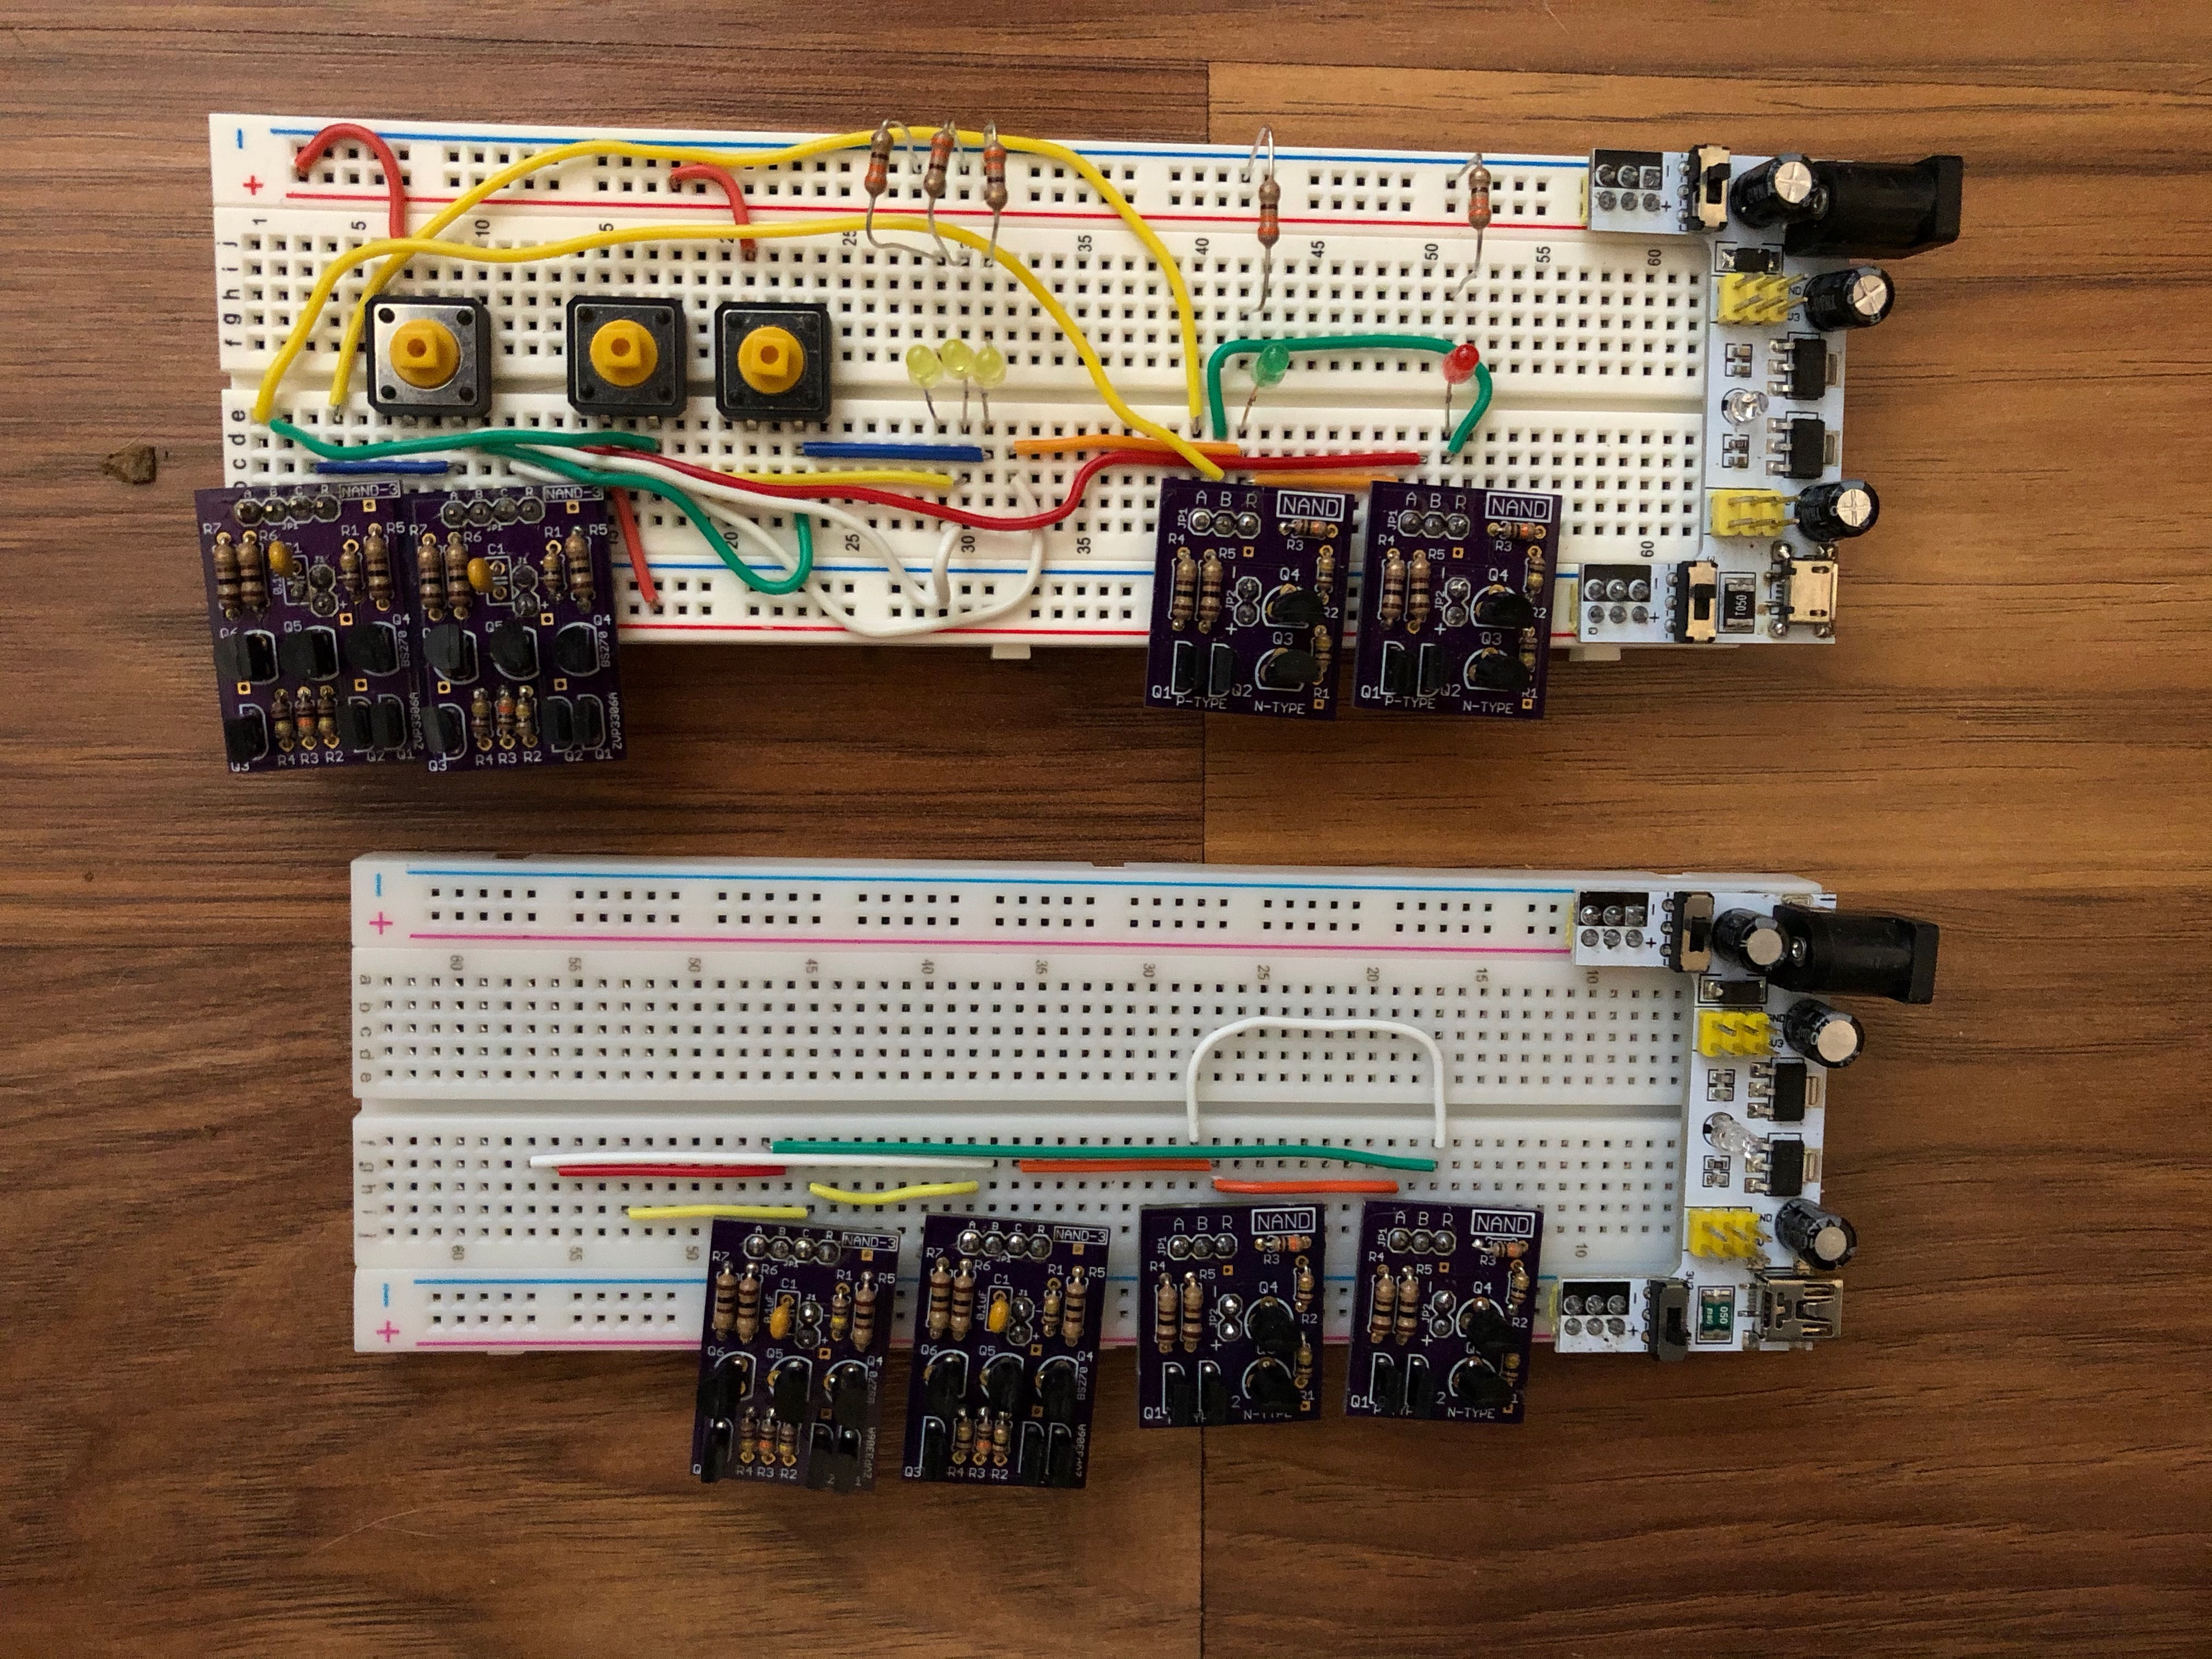
\includegraphics[scale=0.10]{twoflipflops.jpg}
  \caption{Two bits of data storage, using JK flip-flop gates.}
  \end{center}
\end{figure}








%---------------------------
\clearpage
\newpage
\section*{Resistor Chart}
%---------------------------

Resistors are marked with colored bands to make it easy to determine what 
resistance value they have, and how close each individual part's value is 
guaranteed to be to that stated value.


\begin{figure}[!ht]
\begin{center}
\fbox{
\includegraphics[scale=0.60]{resistorchart.png}
}
\caption{A resistor value color band chart. The `tolerance' stripe (how close the value is guaranteed to be to the stated value) is on the right side. }
\label{fig:resistorchart}
\end{center}
\end{figure}

%---------------------------

\clearpage
%\documentclass[12pt]{article}
%\usepackage{tabularx}
%\usepackage{xcolor}
%\usepackage{tikz}
%\usepackage[american, EFvoltages, cuteinductors]{circuitikz}
%\parindent = 0.0pt
%\parskip = 6pt
%\begin{document}

\section{Logic Gate Puzzles}

This section contains some logic puzzles that help you cement your understanding of how using gates together can check inputs and provide outputs according to the questions you specify. The challenges start with simple examples and move to more challenging questions. Every puzzle has an answer provided.


Each puzzle's objective is to solve the question asked, using as few gates as possible. There are many possible solutions, but the solutions focus on one straightforward answer, and sometimes a more clever answer where it exists. All puzzles have similar rules.

\begin{itemize}
\item The solution must only use OR gates, AND gates, and NOT gates
\item There must be a single output to check for the result (that is, you can't ask the user to check three separate AND gates to see if $AB$, $AC$, or $BC$ are ``true'')
\end{itemize}

Some other parameters:
\begin{itemize}
\item You can connect signals to more than one gate at a time if you want to
\item You can connect inputs to each other if it helps
\item You may not have to build a circuit to handle every case
\end{itemize}

\clearpage

\subsection*{Puzzle 1}

Design a circuit that tests to see if A is true but B is false.


\vfill 

\subsubsection*{Answer}

Since there are two \emph{required} conditions, an OR gate won't help us. 
AND gates check if both inputs are equal to 1, but an AND gate will only be useful if it can check if B is 0. 
Another way to express the puzzle is ``A AND NOT B''. 
Because a NOT gate will convert B from ``off'' to ``on'', then the AND gate will work as we want it to.

The solution is the same for the reverse (check for $B=1$ and $A=0$), provided the NOT gate converts the A input instead of the B input.


\begin{figure}[hb!]
\begin{center}

\begin{circuitikz}

% Inputs:
\draw
	(0,5.5) node[ocirc](anode) {} %A node
	(0.25,6.0) node[left] {{\color{red}$A$}} %A label
	
	(0.75,5.5) node[ocirc](bnode) {} %B node
	(1.1,6.0) node[left] {{\color{red}$B$}} %B label
;

% NOT gate:
\draw 
    (2,4.5) node[american not port](notb){}
    node[xshift=5mm, yshift=5mm] {{\footnotesize{$NOT_1$}}} 
;

% AND gate:
\draw 
    (5,3.75) node[american and port, anchor=out](andGate1) {}
	node[xshift=2mm, yshift=-6mm] {{\footnotesize{$AND_1$}}}
    node[ocirc, xshift=2cm](snode) {} %S node
	node[xshift=2cm, yshift=5mm] {{\color{red}$Result$}} % S label
;

% Nets:
\draw[thick](anode) |- (andGate1.in 2);
\draw[blue, thick] (bnode) |- (notb.in 1); 
\draw[thick](notb.out) -| (andGate1.in 1);
\draw (andGate1.out) to (snode);

\end{circuitikz}

\caption{Using discrete gates to test for $A$ AND NOT $B$.}

\end{center}
\end{figure}


\clearpage

\subsection*{Puzzle 2}

Design a circuit that tests to see if A is \emph{different from} B, no matter what value A has. \emph{Hint: the solution to Puzzle 1 is a huge chunk of the answer.}


\vfill

\subsubsection*{Answer}

This challenge asks you to make an XOR gate. Use the solution from Puzzle 1, twice, swapping the NOT gate in one of the ($A$ AND NOT $B$) or ($B$ AND NOT $A$) blocks. Then take the result from each block and merge the result with an OR gate.

\begin{figure}[hb!]
\begin{center}

\begin{circuitikz}

% Inputs:
\draw
	(0,5.5) node[ocirc](anode) {} %A node
	(0.25,6.0) node[left] {{\color{red}$A$}} %A label
	
	(0.75,5.5) node[ocirc](bnode) {} %B node
	(1.1,6.0) node[left] {{\color{red}$B$}} %B label
;

% NOT gates:
\draw
	(2,4.25) node[american not port](nota){}   % not gate #1 input
	(2,1.75) node[american not port](notb){}   % not gate #2 input
;

% AND gates:
\draw
	(4.5,3.75) node[american and port](andGate1) {} % AND gate #1 
	(4.5,2.25) node[american and port](andGate2) {} % AND gate #2 
;

% OR gate:
\draw
	(7.0,3) node[american or port](orGate) {}
;

% From the NOT gates out to the AND gates and OR gate:
\draw[red, thick]
	(nota.out) to[short](andGate1.in 1) % NOT output net goes into andGate1.in 1
;

\draw[orange, thick]	
	(notb.out) to[short](andGate2.in 2) % NOT output net goes into andGate2.in 2
;


\draw[thick]
	(0,3.5) node[circ](atoand1){}
	(atoand1) to [short](andGate1.in 2)
;

\draw[green!50!black, thick]
	(andGate1.out) to [short](5.0,3.75)
	(5.0,3.75)  |- (orGate.in 1)
;

\draw[brown!60!black, thick]
	(andGate2.out) to [short](5.0,2.25)
	(5.0,2.25)  |- (orGate.in 2)
;

\draw[blue, thick]
	(0.75,4.25) node[circ, color=blue](btonot1){}	
	(bnode) |- (nota.in)
;

\draw[thick]
	(0,5.5) |- (notb.in)
	(0,1.75) node[circ](atonot2){}
;

% B input line nets:
\draw[blue, thick]
	(0.75,4.25) to [short](0.75,2.5)
	(0.75,2.52) node[circ, color=blue]{}
	(0.75,2.52) |- (andGate2.in 1)
;

\draw	
% Output nodes:
	(8,3) node[ocirc](snode) {} %S node
	(8.25,3) node[right] {{\color{red}$Result$}} % S label
	(orGate.out) to [short](snode) % S output 
	
% Labeling:
	(1.75,4.85) node[right] {{\footnotesize{$NOT_1$}}} 
	(1.75,1.15) node[right] {{\footnotesize{$NOT_2$}}} 
	(3.5,4.6) node[right] {{\footnotesize{$AND_1$}}} 
	(3.5,1.35) node[right] {{\footnotesize{$AND_2$}}}
	(6.5,3.7) node[right] {{\footnotesize{$OR$}}}
    
    ;

\end{circuitikz}

\caption{Using discrete gates to make an XOR gate. One pair of NOT and AND gates solves for ($A$ AND NOT $B$), while the other pair solves for ($B$ AND NOT $A$). The OR gate returns true if either condition is true.}

\end{center}
\end{figure}

\clearpage

\subsection*{Puzzle 3}

Say you had three inputs $A$, $B$, and $C$, and you want to know when a majority of them are ``on'' or ``true''. The question is simple enough: with three inputs, use connected logic gates in a way that can tell when the majority of inputs (here, that's two of the three) are ``true''. There's a way to represent these conditions in a compact way: 
\begin{itemize}
\item If all of the inputs are off, then the condition can be represented by: $\overline{ABC}$. 
\item When all inputs are on, the shorthand would be $ABC$. 
\item When only A is off, the condition is represented by $\overline{A}BC$. 
\end{itemize}

So a line over the letter indicates ``NOT true", and no line indicates ``true''.

\subsubsection*{Setting Up}

We hinted at the solution above.
The goal is to detect if any two signals are true. 
That means any combination of the three signals that has two or more of them reporting ``yes''. 
How many combinations are there in total?

\begin{enumerate}
\item Each input can be 1 or 0 -- there are exactly two possible states
\item There are three inputs in total, and each can be on or off
\item Each input is not affected by any other input (the inputs are not tied together in any way)
\end{enumerate}

The truth table will have $2 \times 2 \times 2$ (that is, $2^3$) possible combinations. So let's make a table by counting from 0 to 7 in binary. We will assign one of the inputs to each column ($2^0$, $2^1$, and $2^2$).

\renewcommand{\arraystretch}{1.2}

\begin{tabular}{m{2in} m{3in}}

\begin{tabular}{cccc}
\hline
A & B & C & Symbol\\
\hline
0 & 0 & 0 & $\overline{ABC}$\\
0 & 0 & 1 & $\overline{AB}C$\\
0 & 1 & 0 & $\overline{A}B\overline{C}$\\
0 & 1 & 1 & $\overline{A}BC$\\
1 & 0 & 0 & $A\overline{BC}$\\
1 & 0 & 1 & $A\overline{B}C$\\
1 & 1 & 0 & $AB\overline{C}$\\
1 & 1 & 1 & $ABC$\\
\hline
\end{tabular}

&

To cover every possible case, half of of each column will be ``true'' and half will be ``false. For the left-most column (``A''), the first four column values are ``off'' and the next four are ``on''. The right-most column alternates ``on-off'' four times, and the middle column alternates off and on every other row. 


\\
\end{tabular}

\renewcommand{\arraystretch}{1.0}


The table shows us all possible conditions for these three inputs. Now add a results column, showing the answer our logic circuit should produce. Remember, if any two inputs in the row are true, then the result column will be true. Otherwise, the result is false.

\begin{tabular}{m{2in} m{3in}}
\renewcommand{\arraystretch}{1.2}
\begin{tabular}{ccccc}
\hline
A & B & C & Symbol & Result\\
\hline
0 & 0 & 0 & $\overline{ABC}$ & 0\\
0 & 0 & 1 & $\overline{AB}C$ & 0\\
0 & 1 & 0 & $\overline{A}B\overline{C}$ & 0\\
0 & 1 & 1 & $\overline{A}BC$ & 1\\
1 & 0 & 0 & $A\overline{BC}$ & 0\\
1 & 0 & 1 & $A\overline{B}C$ & 1\\
1 & 1 & 0 & $AB\overline{C}$ & 1\\
1 & 1 & 1 & $ABC$ & 1\\
\hline
\end{tabular}

&

The fourth, sixth, seventh, and eighth rows all have two or more inputs set to ``on''. The results (``R'') column is 1/``true'' for these four rows, and 0/``false'' for the rest. 

\\
\end{tabular}
\renewcommand{\arraystretch}{1.0}

The logic can be expressed like this: 

($A$ AND $B$) OR ($A$ AND $C$) OR ($B$ AND $C$) OR ($A$ AND $B$ AND $C$). 

So if any of these individual conditions is true, the result is true.
Note that all three values do not have to be true for the result to be true. Any two true inputs gives the same result as all three inputs being on. So there is no need to specifically test for all three inputs being true.


\clearpage
\subsubsection*{Answer 1}

How can we build a logic circuit to produce this result? Let's start with the example we started above. If we use an AND gate for each of the three combinations of inputs that could produce a result of ``true'', we can then put each of the results into an OR gate, because the output of any AND gate tells us that we should produce a result of ``yes''. We have three outputs, and to this point we haven't discovered that there are three-input gates (heh) so we must use two OR gates to capture all three possible ``majority yes'' voting conditions.

Follow the logic and see if you can convince yourself that the logic is correct.


\begin{figure}[hb!]
\begin{center}
%\documentclass[12pt]{standalone}
%\usepackage[left=1in,right=1in,top=1in,bottom=1in]{geometry} 
%\usepackage{xcolor}
%\usepackage{tikz}
%\usepackage[american, EFvoltages, cuteinductors]{circuitikz}
%
%\begin{document}
%\thispagestyle{empty}

\begin{circuitikz}

% Inputs:
	\draw
		(2,5) 
		node[american and port, anchor=in 2, number inputs = 2](And1){{\color{gray}$\mathsf{AB}$~}}
		node[ocirc, xshift = -3cm, yshift=5.5mm](anode){}
    	node[xshift = -3.4cm, yshift = 6mm](){{\color{red}$A$}}
		node[xshift = 0.9cm, yshift = -0.6cm] {{\footnotesize{$AND_1$}}} 
		[brown, thick](anode) |-  (And1.in 1)
	;

	\draw
		(2,3.0) 
		node[american and port, anchor=in 2, number inputs = 2](And2){{\color{gray}$\mathsf{BC}$~}}
		node[ocirc, xshift = -3cm, yshift=0mm](bnode){}
    	node[xshift = -3.3cm, yshift = 0.0mm](){{\color{red}$B$}}
		node[xshift = 0.9cm, yshift = -0.6cm]{{\footnotesize{$AND_2$}}} 
		(bnode) -|  (And2.in 2)
	;

	\draw
	    (2,0.5) 
		node[american and port, anchor=in 2, number inputs = 2](And3){{\color{gray}$\mathsf{AC}$~}}
		node[ocirc, xshift = -3cm, yshift=0cm](cnode){}
    	node[xshift = -3.3cm, yshift = 0.0mm](){{\color{red}$C$}}
		node[xshift = 0.9cm, yshift = -0.6cm]{{\footnotesize{$AND_3$}}} 
		[blue](cnode) -|  (And3.in 2)
	;



    \draw(6, 4.0) 
        node[american or port, anchor=out, number inputs = 2](Or1){}
        node[xshift = 0.0cm, yshift = -0.5cm]{{\footnotesize{$OR_1$}}}
    ;

    \draw(8.5, 1.75) 
        node[american or port, anchor=out, number inputs = 2](Or2){}
        node[xshift = 0.0cm, yshift = -0.5cm]{{\footnotesize{$OR_2$}}}
       	node[xshift = 1.8cm, yshift = 0.0mm](){{\color{red}$R$}}
       	node[ocirc, xshift = 1.5cm, yshift=0cm](rnode){}
       	(rnode) -- (Or2.out)
    ;


\draw (Or1.out) -| (Or2.in 1);
\draw (And1.out) -| (Or1.in 1);
\draw (And2.out) -| (Or1.in 2);
\draw (And3.out) -| (Or2.in 2);

\draw (anode) node[circ, xshift = 0.5cm](aux1){};
\draw [brown, thick](aux1) |- (And3.in 1);
\draw (bnode) node[circ, xshift = 1.5cm](aux2){};
\draw (aux2) |- (And1.in 2);
\draw [blue](cnode) node[circ, xshift = 2.5cm](aux3){};
\draw [blue](aux3) |- (And2.in 1);

\end{circuitikz}

%\end{document}


\caption{A majority detection circuit using three AND gates and two OR gates. Testing specifically for all three inputs being true can be ignored because the circuit only needs to check for a majority of the inputs.}

\end{center}
\end{figure}

\clearpage

\subsubsection*{Answer 2}
But might there be a more efficient way to do this? That is, could we get by with fewer than three AND and two OR gates?\footnote{Would I even ask this question if the answer was ``no''?}

We can be clever and produce a slightly less straightforward-looking circuit that still accomplishes our goal, but uses fewer resources to get the correct answer. The goal is the same -- figure out if any two of the inputs are ``yes''. 

\begin{enumerate}
\item If ($B$ AND $C$) is true, $A$ does not matter -- the result is ``true''

\item If $A$ is ``true'', either $B$ OR $C$ can be ``true'' to get a ``true'' result.

\end{enumerate}

By connecting inputs $B$ and $C$ to both an OR gate and an AND gate, we can capture these conditions more efficiently. Let's write out the logic:

\begin{enumerate}
\item If ($B$ AND $C$) is true, A does not matter---the result is ``true'' regardless of the value of A (this implies that we can use an OR gate to give a result of true if ($B$ AND $C$) is true.

\item If ($B$ OR $C$) is true, AND A is true, the result is also ``true''
\end{enumerate}

So now it should be clear that by connecting B and C to both an AND gate and an OR gate, we can capture condition (1) with an AND gate; and condition (2) with an OR gate that feeds into an input of an AND gate, with the other input tied to A. 
Each result connects to a second OR gate that gives the result value.
In this way, we can solve the question with two AND gates and two OR gates, reducing our need for one AND gate! 
Not the most exciting game, true, but it's the same sort of puzzle as Sudoku.

\begin{figure}[hb!]
\begin{center}

%\documentclass[12pt]{standalone}
%\usepackage[left=1in,right=1in,top=1in,bottom=1in]{geometry} \usepackage{xcolor, tikz} \usepackage[american, EFvoltages, cuteinductors]{circuitikz}
%\begin{document}
%\thispagestyle{empty}

\begin{circuitikz}

% B input:
\draw
	(-1cm,2.75cm) node[ocirc](bnode) {} % 
	node[left] {{\color{red}$B$}} % 
;


\draw
	(2,5) 
	node[american and port, anchor=in 2, number inputs = 2](And1){}
	node[ocirc, xshift = -3cm, yshift=5.5mm](anode){}
   	node[xshift = -3.4cm, yshift = 6mm](){{\color{red}$A$}}
	node[xshift = 0.9cm, yshift = -0.5cm] {{\footnotesize{$AND_1$}}} 
	(anode) |-  (And1.in 1)
;

\draw
	(0,3.5) 
	node[american or port, anchor=in 1, number inputs = 2](Or1){}
	node[xshift = 0.9cm, yshift = -1.1cm]{{\footnotesize{$OR_1$}}} 
;

\draw
    (2,0.5) 
	node[american and port, anchor=out, number inputs = 2](And2){}
    node[ocirc, xshift = -3cm, yshift=-0.275cm](cnode){}
   	node[xshift = -3.3cm, yshift = -2.5mm](){{\color{red}$C$}}
	node[xshift = -0.7cm, yshift = -0.8cm]{{\footnotesize{$AND_2$}}} 
	(cnode) -|  (And2.in 2)
;

\draw
	(6.0,3.0) 
	node[american or port, anchor=out, number inputs = 2](Or2){}
	node[xshift = -0.6cm, yshift = -0.8cm]{{\footnotesize{$OR_2$}}}
	node[ocirc, xshift=1cm, yshift=0mm](rnode){}
;

\draw
	(Or2.out)
	node [yshift = -3mm, xshift = 8mm](r){{\color{red}$R$}}
;

% B nets:
\draw[blue]
	(bnode) |- (Or1.in 1)
	(bnode) |- (And2.in 1)
;

\draw
    node[circ, yshift=2.3mm]{}
    (cnode) -| (Or1.in 2)
;

\draw (Or2.out) -- (rnode) ;
\draw (Or1.out) -| (And1.in 2);
\draw (And1.out) -| (Or2.in 1);
\draw (And2.out) -| (Or2.in 2);

\end{circuitikz}
%\end{document}


\caption{A majority detection circuit using only two AND gates and two OR gates.}

\end{center}
\end{figure}

% \end{document}

%%%%%%%%%%%%%%%%%%%%%%%%%%%%%%%%%%%%%%%%%%%%%%%%%%%%%%%%%%%%%%%%
\end{document}
%%%%%%%%%%%%%%%%%%%%%%%%%%%%%%%%%%%%%%%%%%%%%%%%%%%%%%%%%%%%%%%%
